\documentclass[oneside,final,14pt,a4paper]{extreport}

\usepackage{tempora} % Times New Roman alike font  

\usepackage{minted} 
\usepackage{setspace} 
\setstretch{1.5} 
\usemintedstyle{bw}
\setminted{fontfamily=txtt}
\newcommand{\haskell}[1]{\mintinline{haskell}{#1}}
\newcommand{\kotlin}[1]{\mintinline{kotlin}{#1}}

\usepackage{vmargin}
\setpapersize{A4}
\setmarginsrb{2.5cm}{2.0cm}{2.0cm}{2.0cm}{0pt}{10mm}{0pt}{13mm}
\usepackage{setspace}
\setstretch{1.5}
\usepackage{indentfirst}
\parindent=1.25cm

%%%%% ADDED TO SUPPORT TT BOLD FACES %%%%
\DeclareFontShape{OT1}{cmtt}{bx}{n}{<5><6><7><8><9><10><10.95><12><14.4><17.28><20.74><24.88>cmttb10}{}
\renewcommand{\ttdefault}{pcr}
%%%%% END %%%%%%%%%%%%%%%%%%%%%%%%%%%%%%% 

\usepackage{atbegshi,picture}
\usepackage[T1,T2A]{fontenc}
\usepackage[utf8]{inputenc}

\usepackage[english]{babel}
\usepackage{textgreek}
\usepackage[backend=biber,style=ieee,autocite=inline]{biblatex}
\bibliography{ref.bib}
\DefineBibliographyStrings{english}{%
  bibliography = {References},}
\setcounter{biburlnumpenalty}{100}
\setcounter{biburllcpenalty}{7000}
\setcounter{biburlucpenalty}{7000}
\usepackage{blindtext}

\usepackage{pdfpages}
\newenvironment{bottompar}{\par\vspace*{\fill}}{\clearpage}
\usepackage{amsmath,amsfonts}
\usepackage{url}
\usepackage{amsthm}
\newtheorem{theorem}{Theorem}
\newtheorem{corollary}{Corollary}
\newtheorem{lemma}{Lemma}
\newtheorem{proposition}{Proposition}
\theoremstyle{definition}
\newtheorem{definition}{Definition}
\theoremstyle{remark}
\newtheorem*{remark}{Remark}
\theoremstyle{remark}
\newtheorem*{example}{Example}

\usepackage{float}
\usepackage{graphicx}
\graphicspath{{figs/}} %path to images
\usepackage{array}
\usepackage{multirow,array}
\usepackage{caption}
\usepackage{subcaption}
\usepackage{hyperref}
\hypersetup{colorlinks=true, linkcolor=black, citecolor=black, urlcolor=black}
\usepackage{paralist}
\usepackage{listings}
\usepackage{zed-csp}
\usepackage{fancyhdr}
\usepackage{csquotes}
\usepackage{color}
% \usepackage{anyfontsize}
% \usepackage{mathptmx}
% \usepackage{t1enc}

\usepackage{chngcntr}
\usepackage{upgreek} 
\usepackage{bm}
\usepackage{hyperref}
\usepackage{booktabs}
\usepackage{multirow}
\usepackage{longtable}
\usepackage[font=singlespacing, labelfont=bf]{caption}
%Hints
\newcommand\pic[1]{(Fig. \ref{#1})} %Ref on figure
\newcommand\tab[1]{(Tab. \ref{#1})} %Ref on table

\setlength{\headheight}{32.0976pt}
\usepackage{enumitem}
\newlist{inlinelist}{enumerate*}{1}
\setlist*[inlinelist,1]{%
  label=(\arabic*),
}

% \setcounter{secnumdepth}{4}
\captionsetup[table]{labelfont={normalfont}, name={TABLE}, labelsep={newline}}
\DeclareCaptionLabelSeparator{figSep}{.\quad}
\captionsetup[figure]{labelfont={normalfont}, name={Fig.}, labelsep=period}
\counterwithin{figure}{chapter}

% \usepackage{titlesec}
% \titleformat{\section}[hang]{\fontsize{20}{24}\selectfont\filcenter}{\Roman{section}}{1em}{}
% \titleformat{\subsection}[hang]{\itshape}{\Alph{subsection}.}{1em}{}[]
% \titleformat{\subsubsection}[runin]{\itshape}{\arabic{subsubsection})}{1em}{}[$:$]
% \titlespacing{\subsubsection}{1em}{1em}{1em}
% \titleformat{\paragraph}[runin]{\itshape}{\alph{paragraph})}{1em}{}[$:$\quad]
% \titlespacing{\paragraph}{2em}{1em}{1em}

\usepackage{placeins} % for \FloatBarrier

\pagestyle{fancyplain}

% remember section title
\renewcommand{\chaptermark}[1]%
	{\markboth{\chaptername~\thechapter~--~#1}{}}

% subsection number and title
\renewcommand{\sectionmark}[1]%
	{\markright{\thesection\ #1}}

\rhead[\fancyplain{}{\bf\leftmark}]%
      {\fancyplain{}{\bf\thepage}}
\lhead[\fancyplain{}{\bf\thepage}]%
      {\fancyplain{}{\bf\rightmark}}
\cfoot{} %bfseries


\newcommand{\dedication}[1]
   {\thispagestyle{empty}
     
   \begin{flushleft}\raggedleft #1\end{flushleft}
}

\begin{document}

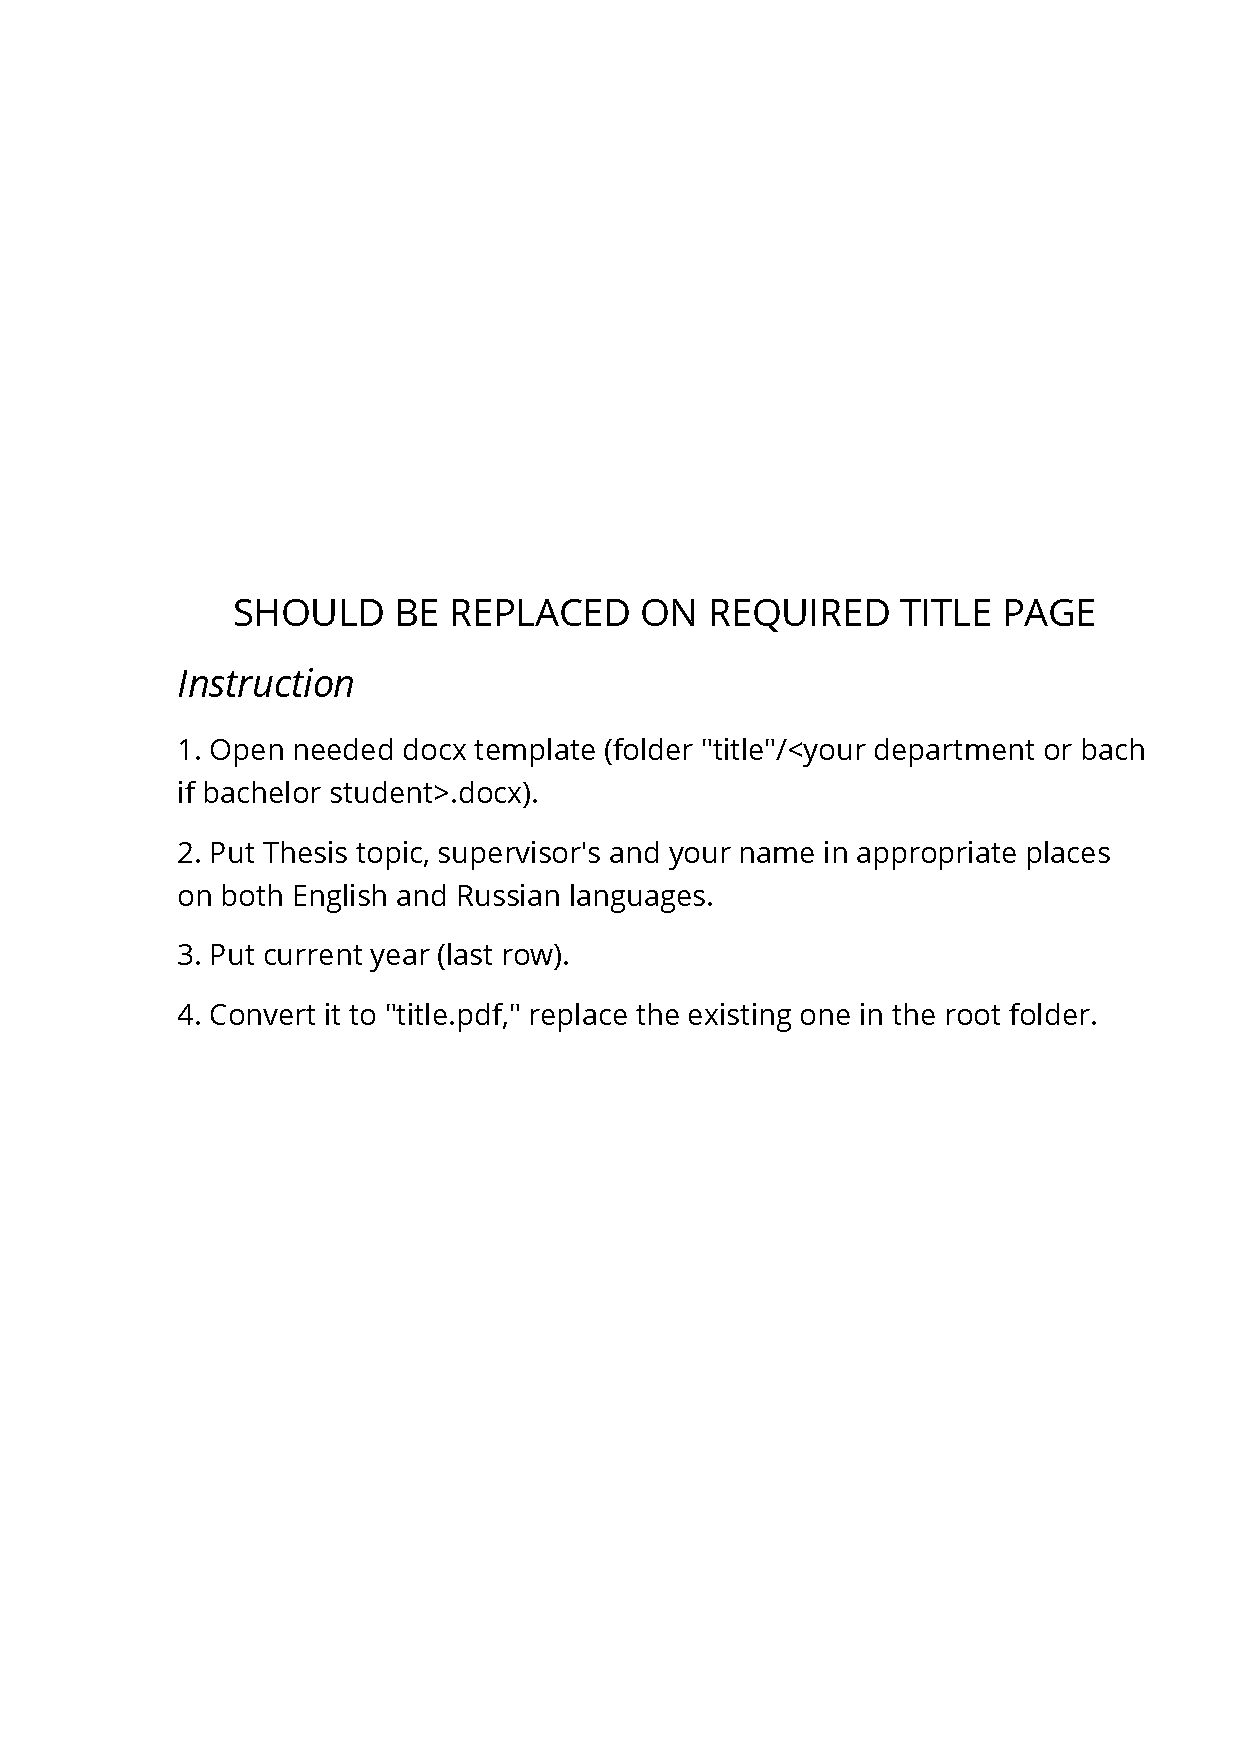
\includepdf[pages=-]{title.pdf}
\tableofcontents
\listoftables
% \listoffigures
\newpage


\chapter*{Abstract}

Name capture during expression substitution remains a critical challenge in programming language implementation and formal verification.
While the Free-Foil framework resolves this issue and automatically generates type-safe syntax, it currently lacks dedicated tooling for rapid IDE integration.
To address this gap, this thesis presents a prototype of an agnostic language server built on Free-Foil that implements core Language Server Protocol (LSP) features: syntax highlighting, diagnostics, hover information, go-to-definition, renaming, and type checking, while requiring little effort from the language author.
Each feature is enabled by implementing a small set of type classes over the language's signature and binders, which keeps tree traversal and scope management inside a reusable library.
A worst-case analysis shows that every server algorithm runs in at most linear time relative to the syntax tree size.
The work also identifies the limitations of the current implementation and directions for extending it.
The prototype is well-suited for educational projects, language prototyping, and rapid integration of domain-specific languages into modern IDEs, with its source code and documentation providing a foundation for further research in automated development tooling.

\chapter{Introduction}
\label{chap:intro}

Language servers are an essential component of modern development environments, providing rich code intelligence features such as code completion, navigation, error checking, and refactoring support. 
The Language Server Protocol (LSP) \cite{lsp}, introduced by Microsoft, has standardized communication between language servers and editors, allowing a common interface for diverse programming environments. 
Implementing a language server from scratch entails a great deal of boilerplate code and similar, repetitive algorithms for every feature, which makes the work slow; more code also tends to mean more bugs that are harder to identify later.
This thesis aims to make the production of a minimal language server a simpler task by moving as much processing as possible into an agnostic framework built on safe and predictable machinery.
It presents a Haskell framework that, given a Free Foil abstract syntax and a set of functions depending on the language-specific signature, produces a language server communicating via LSP that can store the current environment's configuration, update it on file changes, rename symbols, navigate to a symbol's definition, perform type checking, and present informational, diagnostic, and warning messages.

\section{Binding and Scopes}
\label{sec:bindings-and-scopes}

One of the most persistent aspects of language server implementation, as in compiler implementation, is the correct management of variable bindings and scopes. 
In the following Kotlin example, \kotlin{x} cannot simply be replaced with \kotlin{y} in \kotlin{a}'s body when calling \kotlin{a(y)}, because that would mix the local variable \kotlin{x} with the free \kotlin{y}.

\begin{minted}[fontfamily=txtt]{kotlin}
val y = 1
fun a (x: Int): (Int) -> Int = { y -> x + y }
a(y)
\end{minted}

Handling bound identifiers safely and efficiently is a long-studied problem, with approaches ranging from De Bruijn indices \cite{deBruijn1972} through locally nameless and nominal techniques to intrinsically scoped representations; Chapter~\ref{chap:lr} surveys this design space in detail. 
This thesis builds on Free Foil \cite{freefoil2024}, which combines free scoped monads \cite{freemonads2024} with the type-safe, single-pass approach of Foil \cite{foil2023}. 
Free Foil was chosen because, besides being safe and efficient, it generalizes the Abstract Syntax Tree (AST) over a declarative bifunctor signature, so that features such as navigation to a symbol's definition, renaming, and the reporting of scope-related errors can be implemented once, agnostically, and reused for any language with minimal effort.

Free Foil parameterizes the abstract syntax over a \texttt{binder} type and a signature \texttt{sig} that distinguishes regular nodes from those introducing new scopes, indexing every entity by a phantom scope type \texttt{S} so that the Haskell type system statically rejects operations mixing incompatible scopes. 
Capture-avoiding substitution and normalization thus become available out of the box, with no manual renaming or index shifting during tree traversal. 
Crucially, because the signature is a bifunctor it can implement \texttt{Bifoldable}, enabling a universal recursive traversal of any AST regardless of the specific language. 
By requiring additional type classes only when specific signature data is needed, IDE features can be implemented as generic algorithms, turning language server development from a repetitive, language-specific task into a configuration-driven process: a developer provides only a declarative signature and a minimal set of type class instances, while the framework handles scope management, tree traversal, and LSP communication.

The ambition of describing binding once and deriving editor services generically is not new. 
The most developed prior effort is the line of work on scope graphs and the Spoofax/Statix language workbench \cite{scopeGraphs2015,scopesAsTypes2018,spoofax2010}, which specifies name resolution and type checking declaratively and answers them through a runtime search over an extrinsic graph. 
This thesis instead carries the intrinsic, compiler-checked route of Free Foil across the LSP boundary, trading some of the binding breadth of scope graphs for zero-cost, statically verified scope safety. 
Chapter~\ref{chap:lr} develops this comparison (Section~\ref{subsec:scope-graphs-vs-free-foil}), and Chapter~\ref{chap:conclusion} returns to it.

\section{Contribution}
\label{sec:contribution}

This thesis presents a novel, architecture-driven framework for automating the development of language servers by leveraging the Free Foil library. 
The primary contributions are structured around three core aspects: architectural abstraction, developer ergonomics, and computational guarantees.

First, it introduces a modular, language-agnostic architecture that decouples LSP feature implementation from language-specific syntax. 
By building directly on Free Foil's type-safe scope management and capture-avoiding substitution, the framework abstracts away the repetitive, error-prone logic traditionally required for tree traversal, variable tracking, and scope resolution. 
This enables a single codebase to serve as an agnostic language server capable of handling any language defined via a declarative bifunctor signature.

Second, it defines a lightweight, type-class-driven interface that activates core IDE functionalities with minimal developer overhead. 
Through a carefully designed set of type classes---\texttt{RangedSig}, \texttt{FoldablePat}, \texttt{TypeDeductiveSig}, \texttt{TypedSig}, \texttt{TypedPat}, \texttt{HoverableSig}, \texttt{HoverablePat}, \texttt{TokenizableSig}, \texttt{TokenizablePat}, \texttt{DiagnosableSig}, \texttt{DiagnosablePat}---the framework exposes syntax highlighting, diagnostics, go-to-definition, symbol renaming, hover tooltips, and basic type checking. 
A language integrator implements only a declarative AST signature and a small set of type class instances: 14 type-class methods together with the \texttt{buildAsts} function, 15 functions in total. 
All scope management, recursive traversal, and LSP communication are handled automatically by the library, shifting the development paradigm from boilerplate-heavy implementation to configuration-driven setup.

Third, it provides a formal worst-case complexity analysis of all server algorithms, demonstrating that every operation runs in at most linear time relative to the AST size ($O(K)$); position-based queries such as go-to-definition and hover descend a single path and, for fixed-arity grammars, run in time linear in the tree depth ($O(L)$, with $L \leq K$). This guarantees predictable performance and scalability for typical development workflows. 

The framework is validated by two independent example language servers built on it without modifying any core module: LambdaPi, a dependently typed lambda calculus with $\Pi$-types, and Flan, a functional language with let-bindings, pair patterns, and conditionals that exercises the full feature set. 
From a practical standpoint, the proposed framework significantly accelerates the creation of language servers, making it particularly valuable for educational projects, rapid language prototyping, and the integration of domain-specific languages into modern IDEs. 
The thesis also critically evaluates the current implementation, identifying key limitations such as the absence of global namespace resolution, reliance on simple annotation-based type inference (lacking constraint unification), and bulk cache updates upon file modification. 
In response, it outlines concrete directions for future work, including incremental type checking, interval-map indexing for logarithmic-time ($O(\log K)$) position lookups, single-pass tree traversals, and generic default implementations for common LSP features. 
The source code and documentation are provided to serve as a foundational toolkit for further research in automated development tooling.

\section{Thesis Outline}
\label{sec:outline}

The remainder of this thesis is organized as follows. 
Chapter~\ref{chap:lr} reviews the techniques for safe and efficient handling of bound variables, the existing language-agnostic models of name binding and resolution, and the Language Server Protocol. 
Chapter~\ref{chap:met} presents the methodology: the design requirements, the agnostic tree-traversal strategy, and the algorithms behind each supported feature. 
Chapter~\ref{chap:impl} documents the implementation, covering the LSP interface, caching, name-collision handling, and the Flan example integration. 
Chapter~\ref{chap:eval} evaluates the framework against its design criteria and analyzes its automation and computational complexity, together with current limitations and directions for future work. 
Chapter~\ref{chap:conclusion} concludes.

\chapter{Literature Review}
\label{chap:lr}

\section{Name Capture}

The problem of name capture is fundamental in programming language implementation, theorem proving, and formal verification systems. 
When substituting expressions containing bound variables, naïve replacement can lead to variable capture, where a free variable in the substituted term becomes bound, changing the meaning of the expression. 
For example, in lambda calculus, substituting \texttt{y} for \texttt{x} in \texttt{(\textlambda y.x)} would incorrectly yield \texttt{(\textlambda y.y)} if performed naïvely. 
Various approaches to preventing this issue have been developed, each with trade-offs between safety, efficiency, and expressiveness.

The simplest approach, often called "naïve substitution," \cite{bound} uses explicit variable names and requires careful renaming during substitution to avoid capture. While intuitive, this approach is error-prone and inefficient as it requires maintaining and checking against a global context of variable names. De Bruijn indices \cite{deBruijn1972} offer an alternative by replacing names with numeric indices representing binding distance. This solves name capture but creates other issues: terms become difficult to read, and substitution still requires traversing the entire abstract syntax tree (AST) to adjust indices.

Higher-Order Abstract Syntax (HOAS) \cite{HOAS} leverages the host language's binding mechanisms, providing excellent safety but often at the cost of expressiveness when implementing algorithms that need to inspect or transform bound variables. The "rapier" technique used in the Glasgow Haskell Compiler \cite{haskellCompilerSecrets} offers better efficiency by maintaining a stateless local scope and performing capture-avoiding substitution in one pass. However, as noted by Maclaurin et al. \cite{foil2023}, it lacks type safety, making it easy to forget scope extensions or necessary renamings when implementing complex language features.

A separate family, the nominal techniques, treats names themselves as the primitive notion. Building on the nominal sets of Gabbay and Pitts \cite{nominalSets2002}, systems such as FreshML \cite{freshML2003} and Nominal Isabelle \cite{nominalIsabelle2008} provide first-class support for binding, fresh-name generation, and reasoning modulo $\alpha$-equivalence, mainly in functional programming and proof-assistant settings. They offer strong meta-theoretic guarantees but enforce freshness dynamically or through dedicated logical infrastructure rather than through the host language's type system, as the intrinsically typed representations below do.

\subsection{Intrinsic Scoping}

Intrinsic scoping addresses the safety issues of previous approaches by encoding scope information directly in types. With this technique, the type system ensures that all terms are well-scoped by construction, making ill-scoped terms impossible to express. Bird and Paterson's approach \cite{BirdPaterson1999} uses nested data types to represent De Bruijn indices at the type level. For Haskell:

\begin{minted}[breaklines=true]{haskell}
data Exp a
  = Var a
  | App (Exp a) (Exp a)
  | Lam (Exp (Maybe a))
\end{minted}

Here, the type parameter changes when going under a binder (using \texttt{Maybe}), enforcing proper scope extension. While this guarantees safety, it still requires traversing and updating all variables during substitution, impacting efficiency. Additionally, the deep polymorphic recursion consumes significant memory and complicates implementing algorithms that work under binders.

Kmett's \texttt{bound} library \footnote{\url{https://hackage.haskell.org/package/bound}} extends this approach with more flexible representations like locally nameless \cite{Chargueraud2012} and co-de-Bruijn indices \cite{McBride2018}. These variations improve ergonomics but still face fundamental efficiency limitations due to their reliance on explicit index manipulation.

\subsection{The Foil}

The Foil \cite{foil2023} resolves the efficiency-safety trade-off by combining the stateless, single-pass algorithm of the rapier with strong type-level guarantees. 
It implements the Barendregt convention \cite{Barendregt}, claiming all bound variables to be distinct and different from free variables, with type safety.
The Foil achieves this by indexing all expressions, names, and scopes with phantom a type parameter \texttt{S} that represents the current set of in-scope variables. 
\texttt{S} is defined as \haskell{data S = VoidS}

So every entity in the Foil's representation is scope-indexed by a kind \haskell{S}:

\begin{itemize}
    \item \haskell{newtype Name (n :: S)} is the type of a name that belongs to the scope \haskell{n}. The name's underlying representation is a machine-sized integer.

    \item \haskell{newtype Scope (n :: S)} is the type of a scope that contains exactly names of type \haskell{Name n}.
    Similarly to the rapier, it stores an integer map \cite{OkasakiGill1998} to lookup and extend the scope.
    \begin{itemize}
        \item if \haskell{scope1 :: Scope n} and \haskell{scope2 :: Scope n},\\
        then \haskell{scope1 == scope2}
        \item if \haskell{scope :: Scope n} and \haskell{x : Name n},\\
        then \haskell{x `member` scope == True}.
    \end{itemize}

    \item \haskell{newtype NameBinder (n :: S) (l :: S)} is the type of a binder that introduces a single new name. It extends the scope indexed by \haskell{n} into the scope indexed by \haskell{l} with the name contained in it.
    New instances of \haskell{NameBinder n l} can only be created with a \haskell{withFresh} function, which introduces new instances of \haskell{S}-indexed types with rank-2 polymorphism:
    \begin{minted}[breaklines=true]{haskell}
withFresh :: Distinct n 
  => Scope n
  -> (forall l. (Distinct l, Ext n l) => NameBinder n l -> r) 
  -> r
    \end{minted}
\end{itemize}

With these data types, a simply-typed lambda calculus can be represented as the following:
\begin{minted}[breaklines=true]{haskell}
data Expr n where
  Var :: Name n -> Expr n
  App :: Expr n -> Expr n -> Expr n
  Lam :: NameBinder n l -> Expr l -> Expr n
\end{minted}

Here, every expression is indexed with a scope \haskell{s}, as well as variables, which are represented as \haskell{Name n}. It is noteworthy that the body of the lambda expression is indexed with a different scope \haskell{l}, which is exactly the scope \haskell{NameBinder n l} creates. Thus, when going under a binder, the type of the sub-expression changes, imposing a type-level constraint on all the terms within it.

When implementing substitution, the type system ensures:

\begin{itemize}
    \item Substitution is applied to all sub-terms
    \item Scope is properly extended when entering binders
    \item Variables are correctly renamed to avoid capture
\end{itemize}

The Foil's efficiency comes from its \texttt{Sinkable} type class, which allows "sinking" expressions into extended scopes:

\begin{minted}[breaklines=true]{haskell}
sink :: (Sinkable e, Distinct n, Ext n l) => e n -> e l
sink = unsafeCoerce
\end{minted}

Since the Foil uses name-based representation rather than indices, and the underlying representation of names remains unchanged between scopes, this operation is a type-safe zero-cost coercion. This contrasts with De Bruijn-based approaches that must traverse and increment every index.

Despite its advantages, the Foil requires manually writing syntax representations and substitution implementations for each language, creating boilerplate code and limiting reusability across different languages.

\subsection{Free Foil}

Free Foil bridges the gap between generic syntax representation and efficient, type-safe substitution. It combines Kudasov's free scoped monads \cite{freemonads2024} with the Foil to automatically generate well-scoped syntax with capture-avoiding substitution from a language's second-order signature.
The core idea is to parameterize abstract syntax additionally by a bifunctorial signature \texttt{sig} that distinguishes between regular sub-terms and scoped sub-terms (those that may access newly bound variables) and, additionally, by the \texttt{binder}:

\begin{minted}[breaklines=true]{haskell}
data ScopedAST binder sig n where
  ScopedAST :: binder n l -> AST binder sig l -> ScopedAST binder sig n
data AST binder sig n where
  Var :: Name n -> AST binder sig n
  Node 
      :: sig (ScopedAST binder sig n) (AST binder sig n) 
      -> AST binder sig n
\end{minted}

Given a bifunctorial signature \texttt{sig}, the \texttt{AST} data type automatically generates the complete syntax with proper scoping. 
For simply-typed lambda calculus:

\begin{minted}[breaklines=true]{haskell}
data ExprF scope term
  = AppF term term
  | LamF scope
type Expr = AST NameBinder ExprF
\end{minted}

\texttt{CoSinkable} typeclass introduces \texttt{coSinkabilityProof} to support patterns. Given a renaming function and a pattern, it provides a renaming function for the variables bound by the pattern, and a refreshed version of the pattern, hence, making sure variables in patterns are refreshed properly to avoid name capture.

The key innovation is that Free Foil inherits the Foil's efficient substitution algorithm while maintaining complete type safety. The \texttt{Sinkable} instance for \texttt{AST} enables zero-cost scope extensions, and capture-avoiding substitution is derived generically:

\begin{minted}[breaklines=true]{haskell}
newtype Substitution (e :: S -> Type) (i :: S) (o :: S) 
  = UnsafeSubstitution (IntMap (e o))
substitute :: (Bifunctor sig, Distinct o, CoSinkable binder, SinkableK binder) 
  => Scope o 
  -> Substitution (AST binder sig) i o 
  -> AST binder sig i 
  -> AST binder sig o
\end{minted}

Unlike free scoped monads that use nested De Bruijn indices, Free Foil eliminates the need for explicit index manipulation, dramatically improving performance while maintaining the same level of type safety. Benchmarks show that while Free Foil is slightly slower than direct Foil implementations due to the additional layer of abstraction \cite{freefoil2024}, it outperforms nested De Bruijn approaches by orders of magnitude for complex terms.

Additionally, Free Foil supports a template-based approach where scope-safe representations can be automatically derived from naïve AST definitions using Template Haskell, allowing seamless integration with parser generators like BNF Converter (BNFC) \cite{ForsbergRanta2004}.

Because a Free Foil signature is an ordinary bifunctor, traversals over the resulting syntax can reuse standard datatype-generic programming techniques instead of bespoke recursion. Generic traversal has a long lineage in Haskell, from recursion schemes over the fixed point of a functor \cite{recursionSchemes1991} to Scrap Your Boilerplate \cite{syb2003}. Free Foil fits this tradition: deriving \haskell{Bifunctor} and \haskell{Bifoldable} for a signature suffices to fold over every node of any language's syntax, which is exactly the property the IDE features in this thesis rely on to stay language-agnostic.

\section{Language-Agnostic IDE Tooling}
\label{sec:language-agnostic-tooling}

The techniques surveyed so far address name capture from the perspective of representing and manipulating terms inside a single language implementation. 
A complementary line of research asks a broader question: can name binding and resolution be described once, in a language-independent way, so that editor services such as go-to-definition, code completion, and rename refactoring are derived generically rather than re-implemented for every language?
This is precisely the ambition shared by this thesis, and the most developed answer to date is the line of work on scope graphs by the Delft programming languages group, which underpins the Spoofax language workbench \cite{spoofax2010}.

\subsection{Scope Graphs: A Theory of Name Resolution}
\label{subsec:scope-graphs}

Neron, Tolmach, Visser, and Wachsmuth \cite{scopeGraphs2015} observe that name resolution ``cuts across the local inductive structure of programs'': the declaration introduced by a \texttt{let} node may be referenced by an arbitrarily distant descendant, and qualified or imported names escape lexical nesting entirely. 
Defining resolution directly over the abstract syntax tree therefore leads to ad-hoc, per-language symbol-table code that is duplicated across the compiler, the IDE, and any mechanized semantics. 
Their proposal is to factor name resolution into two stages: a language-specific construction of a language-independent scope graph from the AST, followed by a language-independent resolution process over that graph.

A scope graph collapses all AST nodes that ``behave uniformly with respect to name resolution'' into nodes called scopes. 
Each scope carries a set of declarations (binding occurrences $x^D_i$, indexed by their AST position $i$) and references (applied occurrences $x^R_i$). 
Edges between scopes encode visibility: a parent edge $\mathsf{P}$ models lexical nesting, while an import edge models the inclusion of a named scope's contents (used to model ML-style modules, and, elegantly, Java class inheritance as ``the \texttt{extends} clause playing the role of import'').
Resolution is then specified declaratively as a resolution calculus that searches for a path from a reference to a declaration. 
Shadowing, where an inner declaration hides an outer one, is captured not by deleting candidates but by a specificity ordering on paths: a path with fewer parent steps is more specific, local declarations are preferred over imports, and imports over lexical parents. 
A reference resolves to a declaration only if that declaration is visible, that is, reachable via a path that no other resolution shadows. 
The authors give a deterministic, terminating resolution algorithm built from an environment-shadowing operator and prove it sound and complete with respect to the calculus.

Crucially for the goals of this thesis, scope graphs are explicitly designed to support front-end tooling rather than only well-formed programs. 
The calculus deliberately admits ambiguous resolutions (multiple declarations for one reference) and unresolved references (free variables), because ``such programs are the normal case in IDEs and other front-end tools.''
On top of resolution, the authors derive language-independent notions of $\alpha$-equivalence, in which two programs are $\alpha$-equivalent if they are structurally identical up to identifiers and induce the same equivalence classes of positions, and of valid renaming as a renaming that preserves $\alpha$-equivalence, that is, introduces no capture. 
This is exactly the rename-refactoring service an IDE must provide, obtained here as a corollary of the resolution theory rather than as bespoke per-language code.

\subsection{Scopes as Types: From Resolution to Type Checking}
\label{subsec:scopes-as-types}

The original scope-graph framework resolves names but says nothing about types, and it was limited to simple, nominal type systems where a type is identified by a name. 
Van Antwerpen, Bach Poulsen, Rouvoet, and Visser \cite{scopesAsTypes2018} extend the framework with the insight that a type can itself be modeled as a scope. 
A record type, a class, or a parameterized type all bind names internally; by representing such a type as a scope in the graph, the internal structure of types is expressed with the very same generic machinery used for ordinary lexical binding. 
Structural subtyping becomes a visibility edge between scopes, and instantiating a generic type becomes the creation of a fresh scope that refines a type parameter's binding.

To make these specifications executable as type checkers, the authors generalize resolution in two ways and embed it in a constraint language. 
First, plain references are generalized to scope graph queries parameterized by a regular-expression label well-formedness predicate and a per-query visibility ordering, so that different namespaces can obey different visibility policies. 
Second, they introduce \texttt{Statix}, a declarative meta-language in which a language designer writes guarded inference-rule-style constraints that simultaneously construct the scope graph and query it, with unification handling type terms. 
The key engineering contribution is decoupling traversal order from solving order: because constraints are solved by a generic solver rather than during a fixed AST traversal, the language designer is freed from manually staging passes to ``collect information before it is needed'' (for example, binding all members of a recursive group before checking their bodies). 
The solver guarantees sound resolution over the gradually-built graph by tracking which scopes may still be extended and delaying any query that could traverse an incomplete scope. 
The approach is implemented in Spoofax and validated on the simply-typed lambda calculus with records, System F, and Featherweight Generic Java, yielding editors with type checking from a single declarative specification.

\subsection{Comparison with Free Foil}
\label{subsec:scope-graphs-vs-free-foil}

Scope graphs and Free Foil pursue the same overarching goal, a single, language-independent treatment of binding from which tooling can be derived, but they sit at opposite ends of a design axis, and this contrast motivates the present work.

\paragraph{Where correctness is enforced.}
Free Foil encodes scope in the host language's type system: every name, scope, and binder is indexed by a phantom kind \haskell{S}, and the Haskell compiler statically rejects any operation mixing incompatible scopes. 
Ill-scoped terms are unrepresentable, and capture-avoiding substitution is correct by construction. 
Scope graphs, by contrast, use an extrinsic model: the graph is an ordinary data structure built alongside the AST, and resolution is a runtime search whose correctness is established by meta-theoretic proof (soundness and completeness of the algorithm with respect to the calculus) rather than by the type system of the implementation language. 
A bug in the AST-to-graph mapping yields wrong resolutions silently; in Free Foil an analogous mistake is typically a compile-time type error.

\paragraph{Expressiveness of binding.}
This is where scope graphs are clearly ahead. 
The scope-graph calculus natively handles non-lexical binding, including modules, qualified names, transitive and cyclic imports, and class inheritance, through import edges and tunable well-formedness and visibility policies \cite{scopeGraphs2015}, and ``Scopes as Types'' \cite{scopesAsTypes2018} pushes this all the way to structural and parametric type systems. 
Free Foil, building on the Foil \cite{foil2023} and free scoped monads \cite{freemonads2024}, is designed around lexical binding: a binder extends the scope of the subtree it dominates. 
Non-lexical structures are not thereby excluded, however. 
Because \haskell{S} is only a phantom tag on scopes and the binder is an ordinary type parameter, a scope is an unordered set of names by construction, and a global namespace or an import can be encoded indirectly, as a synthetic binder that extends the scope with the relevant names, with a qualified import reducing to a single-name binder. 
What scope graphs provide and Free Foil does not is the resolution machinery itself: import edges, visibility and well-formedness policies, and cross-module path-finding are derived automatically there, whereas here they must be implemented by hand, and cross-module name identity must be tracked manually because names are scope-local and can be transported only along a scope extension. 
Such manual encodings also fall partly outside Free Foil's by-construction guarantees: the compiler still rejects mixing incompatible scopes, but it does not verify that a synthetic binder faithfully models the intended visibility. 
The gap is thus one of prepacked expressiveness and ergonomics rather than of what the \haskell{S}-indexed representation can ultimately encode.

\paragraph{Treatment of erroneous and partial programs.}
Scope graphs are explicitly engineered for the IDE setting: ambiguous and unresolved references are first-class, which is essential for editor services over the incomplete, frequently-broken programs typical of live editing \cite{scopeGraphs2015}. 
Free Foil's intrinsic guarantees assume a well-scoped term; mapping a partially-written or ill-scoped source file into an \haskell{S}-indexed AST requires additional care at the boundary, an issue the implementation chapters of this thesis address directly.

\paragraph{Derived services.}
Both frameworks deliver the same headline IDE features generically. 
Scope graphs derive go-to-definition (path to a declaration), rename (validity defined via $\alpha$-equivalence), and, via Statix, type checking, all from a declarative specification interpreted by a generic solver. 
Free Foil derives capture-avoiding substitution, normalization, and, because a Free Foil signature is a \haskell{Bifunctor} and hence \haskell{Bifoldable}, generic recursive traversal, from a declarative bifunctor signature compiled by the Haskell type checker. 
In other words, Spoofax and Statix achieve genericity through runtime constraint solving over an untyped graph, whereas Free Foil achieves it through compile-time type-level guarantees over a scoped AST.

\paragraph{Positioning of this thesis.}
The two approaches are complementary rather than competing. 
Scope graphs demonstrate the breadth of binding patterns a truly language-agnostic tool must eventually cover and set the standard for IDE-oriented robustness, but they obtain their guarantees through proof and runtime search and are tied to the Spoofax ecosystem. 
This thesis instead asks how far the intrinsic, type-safe route of Free Foil can be carried into a standalone, LSP-based language server: trading some of the breadth of scope graphs (notably non-lexical binding and rich type systems) for zero-cost, compiler-checked scope safety and a configuration-driven implementation that lives in mainstream Haskell tooling rather than a dedicated workbench.

\subsection{Language Workbenches}
\label{subsec:language-workbenches}

Spoofax is one of a broader class of language workbenches, tools built on the premise of ``define a language, get an IDE for free.'' Systems such as Xtext \footnote{\url{https://eclipse.dev/Xtext/}}, JetBrains MPS \footnote{\url{https://www.jetbrains.com/mps/}}, and Rascal \footnote{\url{https://www.rascal-mpl.org/}} let a designer specify a language's grammar, name binding, and semantics, and generate editor support from that specification. The framework of this thesis shares this philosophy but is deliberately narrower: rather than a full workbench with its own meta-languages and environment, it targets the single goal of deriving a standalone LSP server from a Free Foil signature, and operates within ordinary Haskell tooling.

\subsection{Tree-sitter}
\label{subsec:tree-sitter}

A different route to language-agnostic tooling is taken by Tree-sitter \footnote{\url{https://tree-sitter.github.io/tree-sitter/}}, an incremental parsing library that re-parses fast enough for every keystroke and recovers gracefully from syntax errors. From a single declarative grammar it powers syntax highlighting and structural navigation across many editors and dozens of languages. Tree-sitter is, however, purely syntactic: it has no notion of name binding, scope, or types, so semantic services such as go-to-definition or rename must still be built on top of it per language. It is thus complementary to the present work, which is concerned precisely with the scope-aware layer that Tree-sitter leaves out.

\section{Language Server Protocol (LSP)}
\label{sec:lsp}

The Language Server Protocol (LSP) \cite{lsp} standardizes communication between a language server, a process that performs language analysis, and a language client in the editor. 
This section reviews what the protocol defines, focusing on the features implemented by the framework of this thesis, and surveys the libraries used to build servers.

\subsection{Protocol Foundations}
\label{subsec:lsp-foundations}

LSP is built on JSON-RPC: every message is a JSON object exchanged over a transport such as standard input/output or a socket. 
The protocol distinguishes three kinds of messages. 
Requests carry an identifier and expect a matching response, whereas notifications carry no identifier and are fire-and-forget. 
Communication is bidirectional: both client and server may initiate requests and notifications, which is what allows a server to push diagnostics to the editor without being asked.

A session begins with a capability negotiation. 
The client opens with an \texttt{initialize} request advertising the features it supports; the server replies with its own server capabilities, declaring which requests it can answer and configuring options such as how documents should be synchronized. 
Only after the client acknowledges with an \texttt{initialized} notification does normal operation begin. 
This handshake means a server need not implement the entire specification: it offers a subset of features, and the editor adapts to whatever is advertised. 
A symmetric \texttt{shutdown}/\texttt{exit} exchange ends the session.

\subsection{Text Document Synchronization}
\label{subsec:lsp-sync}

A language server does not, in general, read source files from disk. 
Instead the client owns the authoritative, possibly-unsaved contents of every open document and streams changes to the server. 
Three notifications govern this lifecycle: \texttt{textDocument/didOpen} announces a newly opened document together with its full text, \texttt{textDocument/didChange} reports edits, and \texttt{textDocument/didClose} signals that the client no longer tracks it. 
Documents are identified by URIs and carry a monotonically increasing version number so that edits can be ordered unambiguously.

The server chooses, during capability negotiation, how much of a document each change notification carries. 
With full synchronization the client resends the entire document on every edit, whereas incremental synchronization sends only the changed ranges, leaving the server to maintain the document state. 
Full synchronization is simpler to implement at the cost of reprocessing the whole file on each keystroke; this trade-off is directly relevant to the caching and re-analysis strategy discussed in the implementation chapters.

\subsection{Language Features}
\label{subsec:lsp-features}

\paragraph{Positions and ranges.}
Almost every language feature is phrased in terms of source locations. 
LSP encodes a position as a zero-based \texttt{(line, character)} pair and a range as a start--end pair of positions. 
Because these offsets are zero-based and counted in UTF-16 code units rather than Unicode characters, a server must translate between its internal representation and the protocol's convention; parsers that report one-based lines and columns, as is common, require an off-by-one adjustment at the boundary. 
Mapping each abstract syntax tree node to the range of source text it spans is therefore a prerequisite for almost all the features below.

\paragraph{Navigation and editing.}
The \texttt{textDocument/definition} request asks the server to resolve the symbol under the cursor to the location of its declaration, the canonical ``go-to-definition'' service. 
The \texttt{textDocument/rename} request asks for all edits needed to consistently rename a symbol throughout the document; the server returns a workspace edit describing the textual changes. 
Both of these are fundamentally name-resolution queries, which is precisely where intrinsically scoped representations have something to offer.

\paragraph{Informational features.}
The \texttt{textDocument/hover} request returns documentation or type information to display when the cursor rests on a symbol. 
The \texttt{textDocument/semanticTokens} request provides token-level classification for semantic syntax highlighting, allowing the editor to color identifiers according to whether they denote, say, a variable, a function, or a type, which purely lexical highlighting cannot recover. 
Tokens are returned in a compact, delta-encoded integer format relative to the previous token.

\paragraph{Diagnostics.}
Errors and warnings are delivered through \texttt{textDocument/publishDiagnostics}, a server-initiated notification: rather than waiting to be queried, the server pushes a list of diagnostics, each consisting of a range, a severity, and a message, to the client whenever its analysis of a document changes. 
This is the channel through which scope errors, type mismatches, and unbound symbols surface to the user.

\subsection{Libraries for Building Language Servers}
\label{subsec:lsp-libraries}

Because the protocol is verbose and its message types numerous, most servers are built on a library that handles the JSON-RPC framing, message (de)serialization, and lifecycle bookkeeping, leaving the author to supply only the language-specific logic. 
Eclipse LSP4J \footnote{\url{https://github.com/eclipse-lsp4j/lsp4j}} provides this foundation on the JVM and underpins Scala's Metals \footnote{\url{https://github.com/scalameta/metals}} and the Kotlin Language Server \footnote{\url{https://github.com/Kotlin/kotlin-lsp}}. 
For Haskell, the \texttt{haskell/lsp} \footnote{\url{https://github.com/haskell/lsp}} family (including \texttt{lsp-types} and \texttt{lsp-test}) offers type-safe representations of the LSP message types together with the communication machinery, and has been hardened through its use in the Haskell Language Server (HLS). 
The framework presented in this thesis is built on \texttt{haskell/lsp}, delegating protocol handling to it and contributing the layer above: the generic, Free-Foil-based analysis that answers the requests described in Section~\ref{subsec:lsp-features}.

Crucially, these libraries are protocol frameworks, not semantic ones. 
They marshal messages and manage document state, but they impose no model of abstract syntax, name binding, or scope; the language author is left to implement resolution, renaming, and type checking from scratch for every language. 
This is the gap the present work targets: by layering a scope-safe, language-agnostic analysis over a protocol library, the repetitive semantic core of a server is provided once rather than rewritten per language.

\section{Conclusion}

This review examined three threads that together frame the problem this thesis addresses: techniques for safe and efficient handling of bound variables, language-agnostic models of name binding and resolution, and the Language Server Protocol that connects analysis to the editor.

The first thread shows a steady progression from error-prone manual renaming, through De Bruijn indices and nominal techniques, to intrinsically scoped representations. The Foil enforces scope correctness at the type level while retaining the single-pass efficiency of the rapier, and Free Foil generalizes this guarantee to any language described by a bifunctor signature, deriving capture-avoiding substitution and generic traversal without per-language boilerplate. This makes type-safe scoping not merely correct but reusable.

The second and third threads reveal where that reusability has not yet been applied. Scope graphs demonstrate that name resolution, $\alpha$-equivalence, and renaming can be specified once and reused across languages, but they obtain their guarantees through meta-theoretic proof and runtime constraint solving rather than the host type system, and the most complete realization lives inside the Spoofax workbench. The Language Server Protocol, meanwhile, standardizes how such services reach any editor, and a mature ecosystem of libraries handles its message-level concerns, yet these libraries stop at the protocol boundary and impose no model of binding or scope, leaving each language to reimplement resolution, renaming, and type checking from scratch.

A gap therefore remains between the two halves of the picture. The machinery for intrinsically scope-safe, language-agnostic syntax exists in Free Foil, and a standard transport for editor services exists in LSP, but no work connects them: language servers are still typically built on extrinsically scoped ASTs with bespoke per-language logic, vulnerable to subtle binding bugs and to repeated implementation effort. Carrying Free Foil's compile-time scope safety across the protocol boundary into a single, configuration-driven server is the opportunity this thesis pursues, trading the broader binding expressiveness of scope graphs for zero-cost, compiler-checked guarantees and a substantially smaller implementation burden per language.

\chapter{Methodology}
\label{chap:met}

\section{Design Requirements}

The goal of my research is to develop an out-of-box solution for a minimal language server. 
Given a Foil AST and some signature-dependant functions, it has to compile into a binary communicating via LSP. 
I would also like to provide a small example-project demonstrating the integration of such a language server into the Visual Studio Code (VS Code) \footnote{\url{https://code.visualstudio.com/}}, an open-source code editor.

The main criterion is the simplicity for an end user. 
This also means requiring as less boilerplate code as possible. 
So that a person wishing to create a proof assistant or a simple programming language for educational or research purposes could have provided the minimal set of functions, while all the heavy-lifting would have lied on the agnostic languages server's shoulders. 
Specifically, the implementation of LSP methods for symbols definition, renaming, type-checking, code highlighting, producing diagnostic and hover messages. 
All of the methods above could be implemented by juggling a finite amount of functions.

\subsection{Deprioritized Criteria}

The project does not focus on substituting complex enterprise-level language servers, nor does it provide a "swiss knife" for any level of complexity projects. 
Hence, the performance and extensibility are deprioritized.
Though, this doesn't mean the behavior of a resulting language server should be non-customizable and slow. 
Rather it only implies the performance and extensibility must not come in contradiction with the prioritized criteria.

\subsection{Evaluation Criteria}
\label{subsec:evaluation_criteria}

To assess whether the proposed language server framework meets its design goals, the following criteria will be used:

\begin{enumerate}
  \item \textbf{Feature Completeness}: The framework must support essential LSP features including \textit{go-to-definition}, \textit{symbol renaming}, \textit{showing hover and diagnostic messages}, \textit{type checking}, and \textit{syntax highlighting}. 
  Each feature should function correctly when the corresponding user-provided functions are implemented.

  \item \textbf{Minimal Entry Threshold}: The framework must provide dummy implementations for the type classes' functions where possible to minimize time required for the first (featureless) language server launch.
  
  \item \textbf{Correctness}: Symbol resolution must accurately trace variable definitions to their usages within the correct scope.
  
  \item \textbf{Language Agnosticism}: The framework should work with at least two distinct language implementations without modification to the core server logic. 
  This demonstrates the \texttt{binder} and \texttt{sig} parameterization achieves true abstraction.
  
  \item \textbf{Worst-Case Complexity}: While performance is deprioritized, every server operation must run in at most linear time in the size of the syntax tree ($O(K)$). A linear bound is unavoidable for whole-file operations such as syntax highlighting and diagnostics, which must visit every node to produce their output; requiring it of every operation ensures the library introduces no super-linear behavior of its own, while leaving room for individual operations to do better.
  
  \item \textbf{VS Code Integration}: The example project must demonstrate successful integration with Visual Studio Code, with all supported LSP features accessible through the editor's standard interface.
\end{enumerate}

These criteria will be evaluated through the implementation of the example project mentioned in Section~\ref{chap:met}.

\section{Language Server Methods}

\subsection{Building a Tree}

The first operation required for any language server is to build the AST, since it is essentially what is going to be analyzed throughout the course of a user's session. 
Given a language's file extension, finding certain files, converting them into ASTs, and even tracking modifications is relatively easy.
However, parsing the AST must be a user's task since the language server is supposed to know nothing about the syntax of the given language.

Some languages may represent programs as a list of declarations.
From the scope-tracking view, these are programs where the scopes gets injected manually to an expression according to the whole project's context.
The program, hence, is defined as a set of expressions, not a nested structure. 
Scope management in these scenarios becomes more sophisticated compared to the nested one-expression case.
Yet it's still possible to produce a Free Foil AST leaving a single expression representing a whole program afterwards, turning it into a list of expressions each with a distinct scope is also a solution.
In terms of an agnostic language server producing a list of trees from a given \texttt{String} input is a cheap yet powerful modification comparing to limiting it to a single element allowing for more user customizations without a requirement to extend the second-order abstract syntax signature. 

The function producing Free Foil ASTs from a given input is defined as the following:

\begin{minted}[breaklines=true]{haskell}
buildAsts :: String -> [SomeScopeWithAST binder sig]
\end{minted}

\texttt{SomeScopeWithAST} is parametrized by a \texttt{binder} and \texttt{sig} but it also introduces an existential variable \texttt{n} which makes any function referring to the \texttt{SomeScopedAST} independent of the concrete phantom type parameter \texttt{n} while also preserving the relation of the \texttt{AST binder sig n} to the scope \texttt{Scope n}.

\begin{minted}[breaklines=true]{haskell}
data SomeScopeWithAST binder sig where
  SomeScopeWithAST :: (Distinct n) 
    => Scope n 
    -> AST binder sig n 
    -> SomeScopeWithAST binder sig
\end{minted}

\subsection{Agnostic Tree Traversal}
\label{subsec:agnostic_traversal}

A central challenge in building a language-agnostic server on top of Free-Foil is traversing an \texttt{AST binder sig n} without knowing the concrete types of \texttt{binder} or \texttt{sig}.
A term is either a free variable \texttt{Var} or a \texttt{Node} whose immediate children are encoded by the signature:

\begin{minted}[breaklines=true]{haskell}
data AST binder sig n where
  Var :: Foil.Name n -> AST binder sig n
  Node 
    :: sig (ScopedAST binder sig n) (AST binder sig n) 
    -> AST binder sig n
data ScopedAST binder sig n where
  ScopedAST :: binder n l -> AST binder sig l -> ScopedAST binder sig n
\end{minted}

The first type argument of \texttt{sig} carries scoped children, sub-expressions placed under a binder of the form \texttt{ScopedAST binder sig n}, while the second carries plain sub-expressions \texttt{AST binder sig n}.
Without additional constraints, the signature is entirely opaque to the server.

The \texttt{Bifoldable} type class provides the ability to fold over both argument positions of \texttt{sig} in a single pass:

\begin{minted}[breaklines=true]{haskell}
class Bifoldable t where
  bifoldl :: (c -> a -> c) -> (c -> b -> c) -> c -> t a b -> c
\end{minted}

A call to \texttt{bifoldl} dispatches two callbacks, one for scoped children and one for plain sub-expressions, threading an accumulator through all of them.
Applying this recursively yields a fully generic depth-first traversal requiring no knowledge of the grammar:

\begin{minted}[breaklines=true]{haskell}
traverseAST
  :: (Bifoldable sig)
  => (forall n. Foil.Name n -> acc -> acc)
  -> (forall n. AST binder sig n -> acc -> acc)
  -> acc -> AST binder sig n -> acc
traverseAST onVar _ acc (Var name) = onVar name acc
traverseAST onVar onNode acc (Node sig) =
  bifoldl
    (\a (ScopedAST _binder body) -> traverseAST onVar onNode a body)
    (\a subterm -> traverseAST onVar onNode a subterm)
    (onNode (Node sig) acc)
    sig
\end{minted}

The constraint \texttt{Bifoldable sig} is the only structural requirement for a complete read-only walk of the tree.

Complementarily, the \texttt{Bifunctor} type class provides \texttt{bimap}, which transforms both child positions of \texttt{sig} simultaneously:

\begin{minted}[breaklines=true]{haskell}
class Bifunctor t where
  bimap :: (a -> c) -> (b -> d) -> t a b -> t c d
\end{minted}

This enables a generic rewriting pass over the AST, where every node is rebuilt after its children have been transformed:

\begin{minted}[breaklines=true]{haskell}
mapAST
  :: (Bifunctor sig)
  => (forall n. AST binder sig n -> AST binder sig n)
  -> AST binder sig n -> AST binder sig n
mapAST _ (Var name) = Var name
mapAST f (Node sig) = f $ Node $
  bimap
    (\(ScopedAST binder body) -> ScopedAST binder (mapAST f body))
    (mapAST f)
    sig
\end{minted}

When a particular algorithm additionally needs to extract information from a node, such as a source location or a construct's display name, the signature can be required to implement a further type class that exposes that information.

Together, folding with \texttt{Bifoldable}, mapping with \texttt{Bifunctor}, and targeted extraction via ad-hoc type classes cover the full space of operations a language server needs to perform on the AST.
Every server-side algorithm can be formulated as a combination of these, with the constraints serving as a precise, type-checked contract between the generic server and the concrete language implementation.
The server core requires no modification when a new language is plugged in; the user only provides type class instances alongside their concrete \texttt{binder} and \texttt{sig}.

\subsection{Locating a Node}

Mapping a cursor position, a line and column pair, to the narrowest AST node that covers it is the starting point for nearly every language server feature.
Go-to-definition, hover messages, and rename all begin by answering the question of what the user is pointing at.
The server cannot hard-code how location information is stored, because it knows nothing about the concrete grammar, so two type classes expose it from the two structural roles a user type can play.

\paragraph{Making signature nodes locatable.}
The \texttt{RangedSig} class asks a fully-applied signature value to report its source range:

\begin{minted}[breaklines=true]{haskell}
class RangedSig sig where
  range :: sig (ScopedAST binder sig n) (AST binder sig n) -> Maybe Range
  range = const Nothing
\end{minted}

The default returns \texttt{Nothing}, so a user who has not yet annotated any constructor still gets a server that compiles and runs; the position search simply will not descend past un-ranged nodes.

\paragraph{Making pattern nodes locatable.}
Binder patterns have kind \texttt{S -> S -> *}, so \texttt{Data.Foldable} cannot be derived for them.
A dedicated class is therefore needed:

\begin{minted}[breaklines=true]{haskell}
class FoldablePat pat where
  foldrPat :: (SomePattern pat sig -> r -> r) -> r -> pat n l -> r
  rangePat :: pat n l -> Maybe Range
  binderOf :: pat n l -> Maybe (NameBinder n l)
\end{minted}

\texttt{foldrPat} walks the sub-patterns of a composite binder; \texttt{rangePat} returns its source range; and \texttt{binderOf} retrieves the single \texttt{NameBinder} at this level of the pattern, if any.
All three methods have placeholder defaults that produce empty results, keeping the class optional to launch the language server but required to support most of the LSP features.

\paragraph{Pattern structure requirement.}
The return type of \texttt{binderOf} is \texttt{Maybe (NameBinder n l)}, reflecting how Free Foil represents scope transitions.
A binder \texttt{pat n l} moves from scope \texttt{n} to scope \texttt{l} through a single \texttt{NameBinder n l}, introducing exactly one name at that level.
Multiple bound names are accumulated by chaining binder levels: the output scope of one level becomes the input scope of the next.
A pattern that binds several names in parallel must therefore be structured as a linked sequence of single-binder levels rather than a flat node holding several names simultaneously; only then can \texttt{foldrPat} visit each introduced name independently and \texttt{binderOf} return a well-typed \texttt{NameBinder} at each step.

\paragraph{The \texttt{Var} wrapper problem.}
A Free-Foil \texttt{Var} carries only a \texttt{Name}, an integer, and no annotation of any kind.
Source ranges can be attached exclusively to \texttt{Node}s through the signature.
A plain \texttt{Var} is therefore invisible to any position-based search: the server cannot locate it, and neither can it retrieve its position after the fact.

The natural remedy is to introduce a dedicated var-wrapper constructor in the signature: a \texttt{Node} whose sole child is the variable it wraps.
Because the wrapper is a \texttt{Node} it can carry a range; because it has exactly one \texttt{Var} child, the server can reliably extract the underlying \texttt{Name} from it.
The user is responsible for inserting these wrappers when converting concrete syntax to the Free-Foil AST; a language implementation that omits them will find name extraction unreliable, making go-to-definition, hover look-up for variables, and rename non-functional, while features that do not depend on name resolution, such as diagnostics and highlighting, continue to work.

\paragraph{Range testing and the search algorithm.}
With location information in place, testing whether a position falls inside a range reduces to boundary comparisons on lines and columns:

\begin{minted}[breaklines=true]{haskell}
inRange :: Position -> Range -> Bool
inRange (Position l c) (Range (Position x y) (Position x' y')) =
  let startsOK = ((l /= x) || (c >= y))
      endsOK = ((l /= x') || (c <= y'))
  in l >= x && l <= x' && startsOK && endsOK
\end{minted}

The predicate handles positions that share a line with a range boundary by additionally checking the column.

\texttt{findNarrowest} combines \texttt{RangedSig}, \texttt{FoldablePat}, and \texttt{Bifoldable} to walk the AST and return the smallest node or pattern covering the requested position:

\begin{minted}[breaklines=true]{haskell}
findNarrowest :: 
  ( Bifoldable sig
  , RangedSig sig
  , CoSinkable binder
  , FoldablePat binder
  , Distinct n )
  => Position
  -> AST binder sig n
  -> Maybe (Either 
      (SomePattern binder sig, SomeAST binder sig) 
      (SomeAST binder sig))
\end{minted}

The result is \texttt{Nothing} when no ranged node covers the position.
Otherwise a \texttt{Left} value indicates the narrowest match is a pattern (together with its enclosing AST node for context), while \texttt{Right} means it is a plain signature node.
The algorithm uses \texttt{Bifoldable} to fold over the scoped and plain children of each \texttt{Node}, recursing only into children that pass the \texttt{inRange} test, and keeping whichever candidate has the smallest covering range.

Once the narrowest node is found, \texttt{extractName} attempts to read a \texttt{Name} from it by looking for the single \texttt{Var} child a var-wrapper node is expected to contain:

\begin{minted}[breaklines=true]{haskell}
extractName :: (Bifoldable sig, Distinct n, CoSinkable binder)
  => AST binder sig n -> Maybe (SomeName binder sig)
\end{minted}

A naked \texttt{Var} passed directly returns \texttt{Nothing}, because the server expects to receive a \texttt{Node}, but a var-wrapper node yields \texttt{Just} the wrapped \texttt{Name}.
The pair of \texttt{findNarrowest} and \texttt{extractName} is the shared prologue for all name-sensitive operations: locate the narrowest node, then ask whether it wraps a variable.

\subsection{Name Definition and References}
\label{section:name_definition_and_references}

The two most prominent name-sensitive LSP features, go-to-definition and rename, share a common core: given a \texttt{Name} extracted from the node under the cursor, find the binder that introduces it, and then collect every node in the binding's scope that refers back to it.
Both tasks require a traversal that is aware of how scope evolves as it descends the tree.

\paragraph{Locating a definition.}
A \texttt{Name} in Free-Foil is an integer indexed by a phantom scope parameter \texttt{n}.
Membership is cheap: \texttt{n `member` scope} returns \texttt{True} exactly when \texttt{n} belongs to \texttt{scope}.
The definition search exploits this by starting at the tree's root with its initial scope and descending into \texttt{ScopedAST} children, extending the running scope with each binder it crosses.
The moment the extended scope contains the target name, the most recently crossed binder is the one that introduced it, and its associated body is the subtree in which that name is live.

The search is split across two functions.
\texttt{findDefinition} is the entry point.
It first checks whether the name is already a member of the starting scope and returns \texttt{Nothing} if so, because a name that is already free in the current expression has no definition inside this tree:

\begin{minted}[breaklines=true]{haskell}
findDefinition isValid (SomeName n) scope ast
  | n `member` scope = Nothing
  | otherwise =
      findDefinition' isValid (SomeName n) scope ast
\end{minted}

\texttt{findDefinition'} is the recursive worker.
Using \texttt{Bifoldable}, it folds over each \texttt{ScopedAST binder body} child of a \texttt{Node}: the binder is used to extend the running scope, membership is checked, and if the name now belongs to the extended scope the binder and body are returned as the result.
When the name is still absent from the extended scope, the worker recurses into the body.
Plain (non-scoped) children are recursed into without changing the scope at all.

Both functions accept an additional validity predicate:

\begin{minted}[breaklines=true]{haskell}
findDefinition ::
  ( Distinct n
  , Bifoldable sig
  , CoSinkable binder )
  => (forall m .
        sig (ScopedAST binder sig m)
            (AST binder sig m)
        -> Bool)
  -> SomeName binder sig
  -> Scope n
  -> AST binder sig n
  -> Maybe
      ( SomePattern binder sig
      , SomeAST binder sig )
\end{minted}

The predicate tests a fully-applied signature node to decide whether a candidate binder should be accepted.
Its primary purpose is to disambiguate parallel scopes.
Two sibling \texttt{ScopedAST} branches can independently introduce names with the same integer identity (since each starts from the same parent scope).
Without additional filtering, the traversal might return the wrong binder.
A natural disambiguator is range coverage: a binder qualifies only if its enclosing node contains the cursor position, which at most one sibling can satisfy if source ranges are non-overlapping.
The predicate is caller-supplied and language-agnostic; the functions themselves impose no constraint on what criterion is used.

\paragraph{Collecting references.}
After the definition is found, the rename and find-all-references operations need every node inside the binding body that refers to the same name.
Two functions handle this, mirroring the definition-search pair.

\texttt{findRefs'} tests the current node and then recurses into its children.
A node counts as a reference if it is a var-wrapper whose single \texttt{Var} child carries the same integer identity as the target name:

\begin{minted}[breaklines=true]{haskell}
findRefs' ::
  ( Distinct m
  , Bifoldable sig
  , CoSinkable binder )
  => SomeName binder sig
  -> AST binder sig m
  -> [SomeAST binder sig]
\end{minted}

The integer comparison is sound because the binder that introduces the target name is an ancestor of every node in its body, so the name is already in scope throughout the subtree.
Foil's \texttt{withFresh} always allocates an identifier beyond those currently in scope, so it can never reassign the target's identifier to another binder inside the body; and the parallel-sibling collisions discussed in Section~\ref{chap:impl} only reuse identifiers allocated within the body, which are necessarily distinct from the already-in-scope target.
No unrelated occurrence can therefore share the target's identifier.

\texttt{findRefs} is the symmetric counterpart: it skips testing the node it receives and dispatches directly to \texttt{findRefs'} on all children via \texttt{bifoldMap}.
The split avoids double-counting when a caller already holds a root node known to be a reference and is only interested in collecting its descendants.

\paragraph{Composing definition and reference search.}
The two pairs are designed to compose.
A go-to-definition query calls \texttt{findDefinition} to obtain the binder pattern, then extracts its source range via \texttt{FoldablePat}.
A rename query calls \texttt{findDefinition} to obtain the definition's body, passes that body to \texttt{findRefs}, and collects the range of every returned wrapper-node to build the complete set of edit locations.
The same combination is equally applicable to a find-all-references request.
Since neither function depends on any language-specific type class beyond \texttt{Bifoldable} and \texttt{CoSinkable}, both pairs are available for any Free-Foil AST without modification to the core server.
The concrete handler logic that wires these building blocks into LSP responses is discussed in the implementation chapter.

\subsection{Type Checking}
\label{section:type_checking}

Type checking in the agnostic language server follows a bidirectional strategy: type expectations are propagated downward from a parent node to its children, while inferred types are returned upward as results.
The user supplies the language-specific deduction rules; the server handles the recursive descent and name-map bookkeeping.
Three type classes divide this responsibility.

\paragraph{Reading types back.}
Once a node or pattern has been annotated with a type, two simple classes expose that annotation:

\begin{minted}[breaklines=true]{haskell}
class TypedSig sig ty where
  ty :: sig (ScopedAST binder sig n) (AST binder sig n) -> ty
class TypedPat pat ty where
  patTy :: pat n l -> ty
  addPattern :: pat n l -> NameMap n ty -> NameMap l ty
\end{minted}

\texttt{TypedSig} extracts the inferred type from any fully-applied signature node.
\texttt{TypedPat} does the same for binder patterns; its second method, \texttt{addPattern}, extends the running name map with the types of the names the pattern introduces, making them available for type-checking the body.

\paragraph{Specifying deduction rules.}
The central class is \texttt{TypeDeductiveSig}:

\begin{minted}[breaklines=true]{haskell}
class TypeDeductiveSig sig sig' ty binder where
  deduceType
    :: ty
    -> sig
        (ty, ty -> (ScopedAST binder sig' n, ty))
        (ty -> (AST binder sig' n, ty))
    -> sig' (ScopedAST binder sig' n) (AST binder sig' n)
\end{minted}

The first argument \texttt{ty} is the expected type for the node as a whole, namely what the node's context demands.
The second argument is the signature with its children already transformed into continuations: each plain child becomes a function \texttt{ty -> (AST ..., ty)}, and each scoped child becomes a pair of its pattern type together with a similar function over the body.
Calling a child's continuation with some type expectation produces both the recursively-checked subtree and its inferred type.
The implementation of \texttt{deduceType} is therefore a pure decision procedure: given the expected type and the child continuations, decide which type to demand of each child, force those continuations, and assemble the output node with a freshly annotated second field.

\paragraph{Orchestrating the recursion.}
The generic \texttt{typecheck} function ties the classes together:

\begin{minted}[breaklines=true]{haskell}
typecheck ::
  ( Bifunctor sig
  , TypeDeductiveSig sig sig' ty binder
  , TypedSig sig' ty
  , TypedPat binder ty
  , Distinct n
  , CoSinkable binder )
  => NameMap n ty -> ty -> AST binder sig n -> AST binder sig' n
typecheck nm typ = \case
  Var n -> Var n
  Node sig -> Node $ deduceType typ $ bimap
    (\(ScopedAST binder a) -> case assertDistinct binder of
      Distinct ->
        let f = first (ScopedAST binder)
              . check (addPattern binder nm) a
        in (patTy binder, f))
    (check nm)
    sig
\end{minted}

A \texttt{Var} node carries no type annotation and is left unchanged; its type will be looked up in the name map whenever a parent's continuation requests it.
For a \texttt{Node}, \texttt{bimap} converts every child in the raw signature into a continuation: plain children become \texttt{check nm}, which recursively calls \texttt{typecheck} and then reads back the inferred type; scoped children are paired with the pattern type from \texttt{patTy} and wrapped so that calling them extends the name map via \texttt{addPattern} before the recursive descent.
The transformed signature is then handed to \texttt{deduceType}, which contains all language-specific logic.

\paragraph{Example: checking a function application.}
Consider the expression \texttt{(\textbackslash x : Int . x) 42} under the expectation that the whole expression has type \texttt{Int}.
In a concrete implementation, this is an \texttt{AppF} node whose two children are the lambda and the integer constant.
After \texttt{bimap} runs, \texttt{deduceType} receives:

\begin{minted}[breaklines=true]{haskell}
AppF a a'
  xOf   -- :: Type -> (AST ..., Type)
  yOf   -- :: Type -> (AST ..., Type)
\end{minted}

The \texttt{AppF} clause then proceeds as follows:

\begin{minted}[breaklines=true]{haskell}
AppF a a' xOf yOf ->
  let (y, yTy) = yOf anyTypeEmp
      (x, xTy) = xOf (FunType funTypeAnnEmp yTy exTy)
      xReturnTy = case xTy of
        FunType _ _ r -> r
        _ -> anyTypeEmp
      (t, errs) = resolveType exTy xReturnTy
  in AppF a (NodeAnn a' t errs) x y
\end{minted}

First, the argument \texttt{42} is checked with no expectation (\texttt{anyTypeEmp}), yielding type \texttt{Int}.
Then the function \texttt{\textbackslash x : Int . x} is checked under the expectation \texttt{Int -> Int}, constructed from the argument type just inferred and the overall expected type \texttt{Int}.
The lambda confirms type \texttt{Int -> Int}, so its return type is \texttt{Int}.
The last step is to compare the inferred return type against the overall expectation.
This requires a user-supplied \texttt{resolveType} function that takes an expected type and an inferred type and returns the resolved type together with any mismatch errors.
A straightforward implementation simply checks equality:

\begin{minted}[breaklines=true]{haskell}
resolveType :: Type -> Type -> (Type, [String])
resolveType expected inferred
  | expected == anyTypeEmp = (inferred, [])
  | expected == inferred   = (inferred, [])
  | otherwise = (expected,
      ["expected " ++ show expected
       ++ ", got " ++ show inferred])
\end{minted}

When the expected type is absent (\texttt{anyTypeEmp}), the inferred type is accepted outright.
When they match, no error is recorded.
Otherwise, a mismatch message is stored in the annotation's error list, which later surfaces as a diagnostic.
More sophisticated languages may unify or subtype rather than check equality, but the interface is the same: given two types, produce a resolved type and any errors.

\subsection{Code Highlighting}
\label{section:code_highlighting}

Code highlighting is based on semantic tokens: a flat list of tokens, each annotated with a type (keyword, variable, function, number, etc.) and a source range, which the editor colors according to its theme.
Unlike syntax-based highlighting, which operates on raw text, semantic tokens are produced from the fully parsed AST, enabling token types that depend on context, such as distinguishing a local variable from a function name.

\paragraph{Why two type classes are needed.}
An AST has two structurally distinct components that may carry token information: the signature nodes in \texttt{sig} and the binder patterns in \texttt{binder}.
A lambda's keyword token belongs to the node, while the pattern variable's token belongs to the binder.
Because both are opaque to the server, two separate type classes expose them:

\begin{minted}[breaklines=true]{haskell}
class TokenizableSig sig where
  tokenize
    :: sig ScopedASTTokens ASTTokens
    -> [SemanticTokenAbsolute]
  tokenize = const []
class TokenizablePat pat where
  tokenizePat :: pat n l -> [SemanticTokenAbsolute]
  tokenizePat = const []
\end{minted}

Both methods have placeholder defaults that return an empty list, so a user who has not yet implemented highlighting still gets a server that compiles and runs correctly, and the feature degrades gracefully to no highlighting.

\paragraph{Token list types.}
The child positions of \texttt{sig} are replaced by their already-computed token lists before \texttt{tokenize} is called.
This requires naming those replacement types:

\begin{minted}[breaklines=true]{haskell}
type ASTTokens = [SemanticTokenAbsolute]
type ScopedASTTokens = (ASTTokens, ASTTokens)
\end{minted}

\texttt{ASTTokens} stands for the token list produced by a plain child.
\texttt{ScopedASTTokens} is a pair: the first component carries the tokens emitted by the binder pattern (\texttt{tokenizePat}), and the second carries those emitted by the body (\texttt{tokenizeAST}).
Together they give \texttt{tokenize} access to every token from every descendant, in addition to whatever tokens the node itself contributes (e.g.\ keyword punctuation stored in the node's annotation).

\paragraph{Generic traversal.}
The recursive descent is implemented once by the library using \texttt{Bifunctor}:

\begin{minted}[breaklines=true]{haskell}
tokenizeAST
  :: (Bifunctor sig, TokenizableSig sig, TokenizablePat binder)
  => AST binder sig n
  -> [SemanticTokenAbsolute]
tokenizeAST = \case
  Var{} -> []
  Node node ->
    tokenize $ bimap tokenizeScopedAST tokenizeAST node
  where
    tokenizeScopedAST (ScopedAST pat body) =
      (tokenizePat pat, tokenizeAST body)
\end{minted}

\texttt{bimap} replaces every child in the signature simultaneously, substituting scoped children with their \texttt{ScopedASTTokens} pairs and plain children with their \texttt{ASTTokens} lists, before the result is handed to the user-supplied \texttt{tokenize}.
A bare \texttt{Var} contributes no tokens on its own: location and token type are attached to the enclosing var-wrapper node through the signature, which is handled by the \texttt{Node} branch.

\paragraph{Ordering constraint.}
Semantic tokens are encoded as position deltas, where each token is positioned relative to the previous one rather than in absolute coordinates.
A consequence is that any token whose start position precedes the end of the token before it in the list is silently dropped.
The token list produced by \texttt{tokenizeAST} must therefore be in source order.

The \texttt{bimap}-based design delegates ordering responsibility to the user's \texttt{tokenize} implementation.
Given the pre-computed token lists for each child, the user concatenates them in the order they appear in the source.
This is natural: the user knows the grammar and can write the children's lists in left-to-right order directly.
An alternative, collecting all tokens and sorting by position, would also be correct but incurs an \(O(K \log K)\) cost and obscures the structure.
The \texttt{bimap} approach keeps the algorithm \(O(K)\) and lets the user exploit grammatical knowledge to avoid the sort entirely.

\subsection{Diagnostics}
\label{section:diagnostics}

Diagnostics are the inline error, warning, and hint messages that an editor displays alongside source code, such as underlines, gutter icons, and problem-panel entries.
Unlike hover messages, which are produced on demand in response to a cursor position, diagnostics are pushed by the server proactively whenever the contents of a file change.
The server walks the entire AST, collects a flat list of \texttt{Diagnostic} values, and publishes them to the editor in one notification.

\paragraph{Why two type classes are needed.}
The structural reason is identical to that for hover and highlighting.
An AST contains two kinds of opaque components, signature nodes in \texttt{sig} and binder patterns in \texttt{binder}, and the server cannot inspect either without a type class.
A pattern such as a let-binding might carry a type-annotation mismatch diagnostic, while a node such as a function application might carry a return-type error.
Keeping the two roles separate lets the user attach diagnostics to whichever component holds the relevant information:

\begin{minted}[breaklines=true]{haskell}
class DiagnosableSig sig where
  diagnose
    :: sig (ScopedAST binder sig n) (AST binder sig n)
    -> [Diagnostic]
  diagnose = const []
class DiagnosablePat pat where
  diagnosePat :: pat n l -> [Diagnostic]
  diagnosePat = const []
\end{minted}

Both methods default to returning an empty list.
A user who has not yet implemented any diagnostic logic still obtains a server that compiles and runs; the feature degrades gracefully to silence.

\paragraph{What the user provides.}
\texttt{diagnose} and \texttt{diagnosePat} return fully assembled \texttt{Diagnostic} values.
A \texttt{Diagnostic} is a structured LSP record carrying, at minimum, a source range and a human-readable message, and optionally a severity level (error, warning, information, or hint), a diagnostic code, and a source label.
Because the appropriate severity and range differ by construct and by language, the user is responsible for building the record; the server provides no further wrapping.
The type-checking pass described in Section~\ref{section:type_checking} is a natural source of diagnostics: the user-supplied type-resolution function stores any mismatch messages directly in node annotations, from which \texttt{diagnose} can extract them.

\paragraph{Generic traversal.}
The collection pass mirrors the structure used for highlighting.
\texttt{diagnoseAST} uses \texttt{Bifoldable} to visit every node and every binder pattern in a single depth-first walk, accumulating the lists produced at each step:

\begin{minted}[breaklines=true]{haskell}
diagnoseAST ::
  ( CoSinkable binder
  , Bifoldable sig
  , DiagnosableSig sig
  , DiagnosablePat binder )
  => AST binder sig n -> [Diagnostic]
diagnoseAST = \case
  Var _ -> []
  Node n -> diagnose n ++ bifoldMap
    (\(ScopedAST binder a) ->
      diagnosePat binder ++ diagnoseAST a)
    diagnoseAST
    n
\end{minted}

A bare \texttt{Var} contributes nothing; its diagnostic, if any, belongs to the enclosing var-wrapper node in the signature.
For a \texttt{Node}, the traversal first calls \texttt{diagnose} on the node itself to collect any diagnostics the user attached at this level, then uses \texttt{bifoldMap} to recurse into the scoped children, calling \texttt{diagnosePat} on each binder and \texttt{diagnoseAST} on each body, and into the plain children.
The result is a flat list of all diagnostics in the tree.

Running \texttt{diagnoseAST} over every tree stored in the file cache and concatenating the results produces the complete diagnostic list for a file, which the server then publishes in a single \texttt{textDocument/publishDiagnostics} notification.

\subsection{Hover Messages}
\label{section:hover_messages}

Hover messages are the documentation popups an editor displays when the user rests the cursor over a symbol.
They typically show type information, a brief description, or any other language-specific annotation the implementation chooses to expose.
Unlike diagnostics, which the server pushes proactively on every file change, hover content is produced on demand: the editor sends a single request carrying a cursor position, and the server must respond with a \texttt{MarkupContent} value, or nothing if the position does not correspond to a hoverable construct.

The production of a hover message therefore decomposes into two independent steps.
First, the server identifies which AST node the cursor is pointing at by calling \texttt{findNarrowest}, whose algorithm was described in \S\ref{subsec:agnostic_traversal} and builds on the location infrastructure introduced there.
Second, it asks that node what, if anything, it has to say.
The second step is language-specific and is therefore delegated to two type classes, one for each structural role an opaque component can play.

\paragraph{Why two type classes are needed.}
The structural reason mirrors that for diagnostics and highlighting.
Hover-relevant information may reside in a signature node, for instance a function-application node annotated with the inferred return type, or in a binder pattern, for instance a let-binding pattern that stores the declared type of the bound name.
Because the server cannot inspect either component directly, two separate classes expose the relevant content:

\begin{minted}[breaklines=true]{haskell}
class HoverableSig sig where
  hoverData
    :: sig (ScopedAST binder sig n) (AST binder sig n)
    -> [String]
  hoverData = const []
class HoverablePat pat where
  hoverDataPat :: pat n l -> [String]
  hoverDataPat = const []
\end{minted}

Both methods default to the empty list, so a user who has not yet implemented hover support still obtains a server that compiles and runs; the feature degrades gracefully to silence.

\paragraph{What the user provides.}
\texttt{hoverData} and \texttt{hoverDataPat} return a list of strings, namely the lines to display for that construct.
The user need not deal with the LSP wire format: the library concatenates these lines into a single Markdown message and wraps it as the \texttt{MarkupContent} value the protocol expects, so the user supplies only the content.
The type-checking pass described in Section~\ref{section:type_checking} is a natural source of that content: the annotation stored on a node after type-checking already contains the inferred type, which \texttt{hoverData} can return as a line directly.

\paragraph{Producing the message.}
Once \texttt{findNarrowest} has identified the construct under the cursor, the server asks it for content directly: if the narrowest match is a binder pattern it calls \texttt{hoverDataPat}, and if it is a signature node it calls \texttt{hoverData}.
A var-wrapper node needs no special treatment, because type checking annotates each node in place and the var-wrapper already carries the information to surface (typically the variable's inferred type), so \texttt{hoverData} returns it without any separate definition lookup.
The lines returned by whichever method fired are concatenated into a single Markdown message and sent to the editor; an empty result yields no hover, which the editor interprets as "nothing to show here."
The server core requires no modification when a new language is plugged in; the user only provides \texttt{HoverableSig} and \texttt{HoverablePat} instances alongside their concrete \texttt{binder} and \texttt{sig}.

\chapter{Implementation}
\label{chap:impl}

\section{LSP Interface}

The Haskell LSP library \footnote{\url{https://github.com/haskell/lsp}} allows to easily run a language server and define its behavior using a list of handlers. 
A handler is a function acting in response to a request body.
The library defines a finite amount of events which can be triggered by a notification or manual request, which, in terms of handlers are all, eventually, just events triggering a consequent response function.
The project uses the following handler-functions:

\begin{itemize}
\item \texttt{Initialized} is triggered on language server initialization; it builds the initial AST cache for all files in the workspace and publishes diagnostics.
\item \texttt{TextDocumentDidOpen} is triggered when a file is opened in the editor; it publishes diagnostics for the newly opened file.
\item \texttt{TextDocumentDidChange} is triggered on every in-editor edit; it rebuilds the AST for the changed file using a debounced timer and publishes updated diagnostics.
\item \texttt{WorkspaceDidChangeWatchedFiles} is triggered when watched files on disk change; it rebuilds the full workspace cache and republishes diagnostics for every file.
\item \texttt{TextDocumentDefinition} is triggered when the user requests navigation to the definition of a symbol under the cursor.
\item \texttt{TextDocumentRename} is triggered when the user initiates a rename operation on a symbol.
\item \texttt{TextDocumentSemanticTokensFull} is triggered when the editor requests semantic highlighting tokens for an entire file.
\item \texttt{TextDocumentHover} is triggered when the user hovers over a symbol and requests contextual information such as an inferred type.
\end{itemize}

\subsection{Language Server Configuration}

The library's public entry point is \texttt{runLanguageServer}, which accepts a single value of type \texttt{LSConfiguration}:

\begin{minted}[breaklines=true]{haskell}
data LSConfiguration binder sig = LSConfiguration
  { fileExtension :: String
  , buildAsts :: String -> [SomeScopeWithAST binder sig]
  }
\end{minted}

These two fields are the only strictly mandatory inputs.
\texttt{fileExtension} names the file extension whose files the server should watch (e.g.\ \texttt{"flan"}), and \texttt{buildAsts} converts raw file text into a list of scope-rooted ASTs, one per top-level declaration or independent scope root.

The remainder of the feature set is controlled entirely by type class instances on \texttt{binder} and \texttt{sig}.
Most classes carry a default no-op implementation, so an integrator can enable features incrementally by providing non-trivial instances.
The type-checking classes, \texttt{TypeDeductiveSig}, \texttt{TypedSig}, and \texttt{TypedPat}, are an exception: because they are parameterized over an unknown type \texttt{ty} that the library cannot infer or default, they require a complete user-supplied implementation.
Table~\ref{tab:ls_features} summarizes which instances unlock which editor features.

\begin{table}[h]
\centering
\begin{tabular}{ll}
\hline
\textbf{Instance(s)} & \textbf{Editor feature} \\
\hline
\texttt{RangedSig}, \texttt{FoldablePat} & Go-to-definition, rename \\
\texttt{TypeDeductiveSig}, \texttt{TypedSig}, \texttt{TypedPat} & Type checking \\
\texttt{HoverableSig}, \texttt{HoverablePat} & Hover messages \\
\texttt{DiagnosableSig}, \texttt{DiagnosablePat} & Diagnostic messages \\
\texttt{TokenizableSig}, \texttt{TokenizablePat} & Semantic token highlighting \\
\hline
\end{tabular}
\caption{Type class instances and the LSP features they enable.}
\label{tab:ls_features}
\end{table}

The \texttt{Bifunctor} and \texttt{Bifoldable} instances are structural requirements inherited from Free Foil and are not specific to any language server feature.
\texttt{F.CoSinkable} is likewise a Free Foil constraint on the binder type required for scope extension during name traversal.

\subsection{Building a Tree}

The \texttt{LSP.Server.Core} module provides a function \texttt{getRootPath} fetching the root path of the current workspace.
Using \texttt{globDir} from the \texttt{System.FilePath.Glob} module it is then possible to collect all files whose extension matches \texttt{fileExtension} from the \texttt{LSConfiguration}.
The \texttt{buildAsts} field, also supplied by the user via \texttt{LSConfiguration}, converts each file's text content into a list of \texttt{SomeScopeWithAST} values, one per top-level declaration or independent scope root.
The resulting pairs of file path and program store are inserted into the cache.

\section{Caching}

The ASTs produced on initialization are cached for later usage. 
Every watched files change triggers ASTs rebuild.

The cache is defined as a separate module independent of Free Foil which is deliberately done to foster modular design and future extensibility to adapt caching to more complex scenarios.
Caching is implemented using Software Transactional Memory (STM) \footnote{\url{https://hackage.haskell.org/package/stm}}.
The program's environment stores a mutable variable \texttt{LangStore ast} parametrized by the final AST type, \texttt{SomeScopedAST binder sig} in the current implementation.
\texttt{LangStore} stores a \texttt{Map} connecting \texttt{FilePath}s to \texttt{LangProgramStore}s, each, essentially, storing the list of ASTs:

\begin{minted}[breaklines=true]{haskell}
newtype LangProgramStore ast = LangProgramStore
  { langAst :: [ast]
  }
newtype LangStore ast
  = LangStore (Map FilePath (LangProgramStore ast))
data LangEnv ast = LangEnv
  { store :: TVar (LangStore ast)
  , debounceTimers :: TVar (Map Uri ThreadId)
  , lspEnvRef
      :: IORef (Maybe (LanguageContextEnv ()))
  }
\end{minted}

The \texttt{store} field holds the cached ASTs protected by an STM transactional variable.
The \texttt{debounceTimers} field maps each open document URI to the \texttt{ThreadId} of a pending rebuild timer, allowing the server to cancel a superseded rebuild when the user types again before the delay expires.
The \texttt{lspEnvRef} field stores the LSP server environment as an \texttt{IORef} so that the debounce thread, which runs outside the \texttt{LSP} monad, can access it to push diagnostics after the rebuild completes.

\paragraph{Why \texttt{IORef (Maybe \ldots)} is necessary.}
The \texttt{runServer} callback accepts a \texttt{ServerDefinition} whose \texttt{staticHandlers} field is evaluated before the LSP handshake takes place.
The \texttt{LanguageContextEnv}, the value needed to run \texttt{runLspT} and send notifications, is only produced inside the \texttt{doInitialize} callback, which fires after the client's \texttt{initialize} request arrives.
The debounce thread, however, is spawned from a handler that was registered earlier, so there is a window during which the thread could in principle execute before \texttt{doInitialize} has stored the environment.
Using a plain \texttt{IORef} containing the fully-initialized value would require the environment to exist at construction time, creating a chicken-and-egg dependency.
\texttt{IORef (Maybe (LanguageContextEnv ()))} resolves this: the reference is initialized to \texttt{Nothing}, then atomically overwritten with \texttt{Just env} inside \texttt{doInitialize}.
The debounce thread reads the reference and exits silently when it finds \texttt{Nothing}, a case that is only possible during the brief initialization window, and proceeds normally once \texttt{Just env} is available.

The \texttt{handleDidChange} handler therefore does not rebuild the cache immediately.
Instead, it calls \texttt{debounceRediagnose}: any existing timer for the document is cancelled, and a new thread is spawned that waits 500 milliseconds before rebuilding the AST, publishing diagnostics, and requesting a semantic-token refresh.
This prevents redundant rebuilds on every keystroke while keeping the IDE's feedback responsive.

The caching module also defines the \texttt{LSP} monad alias used throughout the server:

\begin{minted}[breaklines=true]{haskell}
type LSP ast = LspT () (ReaderT (LangEnv ast) IO)
\end{minted}

\subsection{Name Collisions}

The definition-search algorithm described in Section~\ref{section:name_definition_and_references} uses \texttt{extendScopePattern} to grow the running scope as it crosses each binder, and checks name membership to detect when a binder introduces the target name.
A subtle issue arises when two or more \texttt{ScopedAST} children of the same \texttt{Node} are siblings, that is, when the signature contains parallel scoped branches.
Because each branch starts from the same parent scope and Foil's \texttt{withFresh} picks the next integer past the current maximum, both branches independently extend the scope by the same integer:

\begin{minted}[breaklines=true]{haskell}
myFunction = -- Scope n  (e.g. {})
  ( \x -> doSmth1 x  -- Scope l1 = {0}
  , \y -> doSmth2 y  -- Scope l2 = {0}
  , \x -> doSmth3 x  -- Scope l3 = {0}
  )
\end{minted}

All three binders produce integer identity 0; the scopes \texttt{l1}, \texttt{l2}, and \texttt{l3} are equal as integer sets.
Without further information, \texttt{findDefinition'} using \texttt{bifoldr} would return the first sibling that passes the membership check, which may not be the one containing the cursor.
Comparing the raw source names stored in the AST would still confuse the first and third branches (both named \texttt{x}), so that is not a solution either.

The chosen approach is to thread a validity predicate through \texttt{findDefinition'}.
When the definition search encounters a candidate \texttt{ScopedAST binder body}, it applies the predicate to the node that encloses it before accepting the result.
For go-to-definition and rename, the predicate is \texttt{nodeCovers pos}: a candidate is valid only if its surrounding signature node's source range contains the cursor position \texttt{pos}.
Since \texttt{findNarrowest} has already established that the cursor falls inside the var-wrapper being queried, and since non-overlapping source ranges ensure that at most one of the parallel branches can contain the cursor, the predicate admits exactly the correct branch.
No extra traversal or subtree search is required; the same single pass that searches for the binder simultaneously discards the wrong siblings.

An alternative that was considered but not adopted is to make name generation aware of parallel branches during AST construction.
A customized scope type \texttt{OffsetScope} could carry an integer offset representing how many names have already been allocated by preceding sibling branches, producing globally distinct integers:

\begin{minted}[breaklines=true]{haskell}
toAst :: Distinct n
  => OffsetScope n
  -> Map String (Name n)
  -> RawTerm
  -> (MyAst n, Int)
toAst scope env = \case
  RawPair l r ->
    let (astL, lShift) = toAst scope env l
        (astR, rShift) =
          toAst (shiftScope scope lShift) env r
    in (Node (Pair astL astR), rShift)
\end{minted}

This approach eliminates collisions at the source but introduces a coupling between sibling branches: each branch's scope depends on the names allocated by all preceding siblings, which prevents independent (or parallel) construction of the child nodes.
It also requires replacing Foil's standard \texttt{withFresh} with a custom variant throughout the user's AST builder.
The position-based predicate approach requires no modifications to either the library or the user's AST construction code, keeping the integration surface small.

\section{Example Project}

The agnostic language server was tested by integrating it with two toy programming languages: LambdaPi, a dependently typed lambda calculus with $\Pi$-types, and Flan (Functional LANguage).
Flan exercises the full feature set of the library: type checking, diagnostics, hover messages, semantic highlighting, go-to-definition, and rename.
It is the primary integration example.

\subsection{Signature and Annotations}

Flan is a strictly typed functional programming language with lambda abstraction, let-bindings, pairs, conditionals, and integer, string, and boolean literals.
Its signature has two annotation type parameters: \texttt{a} for source positions and \texttt{a'} for node-level derived data:

\begin{minted}[breaklines=true]{haskell}
data FlanF a a' s t
  = VarF a a' t String
  | AppF a a' t t
  | LamF (LamAnn a) a' s
  | LetF (LetAnn a) a' s s
  | PairF (PairAnn a) a' t t
  | IfF (IfAnn a) a' t t t
  | ConstF a a' FlanConst
  | ErrorF a a' String
\end{minted}

The \texttt{a} parameter (a BNFC source position) is present on every constructor; for nodes that carry multiple keywords, such as \texttt{LamF}, which has a lambda token and a return-type annotation token, a dedicated record (\texttt{LamAnn}, \texttt{LetAnn}, etc.) groups the per-keyword positions.
The \texttt{a'} parameter is the node annotation used for derived information.

AST construction proceeds in two phases.
In the first phase both parameters are instantiated with the raw source position type \texttt{PosAnn}, yielding \texttt{FlanF PosAnn PosAnn}.
In the second phase the type-checker replaces \texttt{a'} with \texttt{NodeAnn}:

\begin{minted}[breaklines=true]{haskell}
data NodeAnn
  = NodeAnn (Maybe (Int, Int)) FlanType' [String]
\end{minted}

\texttt{NodeAnn} stores the node's end position (used to construct a \texttt{Range} together with the start position in \texttt{a}), its inferred type, and any type-error messages accumulated during type checking.
The final AST has type \texttt{FlanF PosAnn NodeAnn} and carries both positional and type information without requiring a separate pass.

Flan's binder is \texttt{FlanPattern}, a recursive algebraic type that supports wildcard, variable, and pair patterns.
Free Foil's \texttt{CoSinkable} typeclass is derived for it, and the library's pattern-binding machinery allows binding zero, one, or several names in a single node without any changes to the core server.

\begin{minted}[breaklines=true]{haskell}
data FlanPattern a ty (n :: S) (l :: S) where
  PatternWildcard :: a -> a -> ty
    -> FlanPattern a ty n n
  PatternVar :: a -> a -> ty -> String
    -> NameBinder n l -> FlanPattern a ty n l
  PatternPair :: PatternPairAnn a -> a -> ty
    -> FlanPattern a ty n i
    -> FlanPattern a ty i l
    -> FlanPattern a ty n l
\end{minted}

\paragraph{Framework requirements on user-defined types.}
These two definitions satisfy the two structural requirements the framework imposes on user-defined AST types.
\texttt{VarF} serves as the var-wrapper: it is a \texttt{Node} constructor whose single plain child is a variable occurrence, giving the server a range-bearing handle on every name use in the source.
\texttt{PatternPair} chains its two sub-patterns through an intermediate scope \texttt{i} rather than storing two binders in a single flat constructor.
This ensures that \texttt{binderOf} can return a single \texttt{NameBinder} at each level and that \texttt{foldrPat} can walk the pattern recursively, extracting one name per step.
A language implementation that represents variable occurrences as bare \texttt{Var} nodes, or that stores multiple binders side-by-side in a single flat pattern constructor, cannot satisfy the \texttt{FoldablePat} and \texttt{RangedSig} contracts; go-to-definition, hover look-up, and rename will be non-functional for those constructs.

\subsection{Type Class Instances}

To activate the full feature set, the Flan integration implements the following type class instances defined by the library:

\begin{itemize}
\item \texttt{RangedSig (FlanF PosAnn NodeAnn)} and\\
\texttt{FoldablePat (FlanPattern PosAnn FlanType')}, required for\\
go-to-definition and rename; they supply source ranges for nodes and binders.
\item \texttt{TypeDeductiveSig}, \texttt{TypedSig}, and \texttt{TypedPat} together describe the bidirectional type-checking rules used to populate \texttt{NodeAnn} with the inferred type.
\item \texttt{DiagnosableSig} and \texttt{DiagnosablePat} collect type errors and unbound-symbol errors stored in \texttt{NodeAnn} into LSP \texttt{Diagnostic} values.
\item \texttt{HoverableSig} and \texttt{HoverablePat} construct hover content from the inferred type and error messages stored in each node's \texttt{NodeAnn}.
\item \texttt{TokenizableSig} and \texttt{TokenizablePat} produce a list of \texttt{SemanticTokenAbsolute} values, assigning token types (variable, function, keyword, number, string) to each sub-expression and keyword token.
\end{itemize}

The entry point wires everything together via \texttt{LSConfiguration}:

\begin{minted}[breaklines=true]{haskell}
runFlanLS :: IO ()
runFlanLS = runLanguageServer LSConfiguration
  { fileExtension = "flan"
  , buildAsts = buildAsts'
  }
\end{minted}

where \texttt{buildAsts'} invokes the BNFC-generated lexer and parser, converts the concrete syntax tree to a Free-Foil AST using the position annotation, and then applies the type-checker to produce the fully-annotated \texttt{NodeAnn} tree.

\subsection{Visual Studio Code Demo}

A minimal Visual Studio Code extension hosts the compiled Flan language server executable and registers it for \texttt{.flan} files.
The extension requires no language-specific logic: it forwards all LSP traffic to the server process.
Through this setup the extension demonstrates go-to-definition, rename, hover with inferred types, squiggly-line diagnostics for type errors and unbound symbols, and syntax highlighting driven by semantic tokens, all enabled by the type class instances above, with no additional hand-written IDE glue.
\chapter{Evaluation and Discussion}
\label{chap:eval}

This chapter assesses the agnostic language server framework against the evaluation criteria established in Section~\ref{subsec:evaluation_criteria}, analyzes the automation it delivers and the computational cost of its algorithms, and identifies current limitations together with directions for future work.

\section{Evaluation against Design Criteria}
\label{sec:eval_criteria}

\subsection{Feature Completeness}

The framework supports all six features from the criterion: go-to-definition, symbol renaming, hover messages, diagnostics, type checking, and syntax highlighting (Table~\ref{tab:ls_features}).
Each is activated by the corresponding type class instances.
The Flan language server exercises all six simultaneously: go-to-definition and rename resolve variable uses to their introducing binders; hover messages display inferred types; diagnostics surface type errors and unbound symbols; semantic tokens drive syntax highlighting in VS Code.

\subsection{Minimal Entry Threshold}

Every method in the non-type-checking classes carries a default returning a neutral value, so the only strictly mandatory inputs are \texttt{fileExtension} and \texttt{buildAsts} in \texttt{LSConfiguration}.
Features degrade gracefully: supplying only \texttt{RangedSig} and \texttt{FoldablePat} immediately enables go-to-definition and rename; each subsequent pair of instances adds the next feature without touching what is already working.
The type-checking classes are a partial exception: because they are parameterized over a user-supplied type \texttt{ty} the library cannot default, omitting them simply means no type-checking support, and all other features are unaffected.

\subsection{Correctness}

Scope-tracking correctness rests on two mechanisms.
Free Foil's phantom type parameter \texttt{n~::~S} makes scope violations a compile-time error: a \texttt{Name n} cannot be compared against a \texttt{Scope m} for a different \texttt{m}, so the server inherits these guarantees for free.
The parallel-scope collision problem, in which sibling \texttt{ScopedAST} branches independently produce names with the same integer identity, is resolved by the position-based validity predicate in \texttt{findDefinition}: because source ranges are non-overlapping, at most one sibling covers the cursor, and only that branch is accepted.
This scope-level correctness is what Free Foil enforces by construction; resolving a name to its definition additionally relies on the structural contracts of Sections~\ref{subsec:agnostic_traversal} and~\ref{chap:impl}, namely var-wrapper nodes around variable occurrences and single-binder-per-level patterns, which the library cannot verify and which the integrator must honor for go-to-definition, rename, and variable hover to function.

\subsection{Language Agnosticism}

Two language servers were built on the library without modifying any core module: LambdaPi (a dependently typed lambda calculus with $\Pi$-types) and Flan (a functional language with let-bindings, pair patterns, and conditionals).
Their signature constructors, binder types, parsers, and type systems share no code; the integration surface in each case consists only of type class instances and the two \texttt{LSConfiguration} fields.

\subsection{Worst-Case Complexity}

The criterion requires every server operation to run in at most linear time in the AST size ($O(K)$).
This is satisfied: the analysis of Section~\ref{sec:complexity} shows that every handler is bounded by $O(K)$, and the library introduces no super-linear step of its own.

Several operations do better than this worst case, which is a welcome bonus rather than a requirement.
Position-only queries, hover and go-to-definition, descend a single root-to-target path instead of the whole tree, so for fixed-arity grammars they run in $O(L)$ in the tree depth (Section~\ref{sec:complexity}); since $L \leq K$, and substantially so for shallow, wide trees, this is a real improvement where it applies.

As subjective corroboration, timing via VS Code's LSP debug log shows individual handler responses in the range of 10 ms on sample Flan programs, which is fast enough to feel instantaneous in the editor.
This is not a controlled benchmark, but together with the complexity bounds it indicates that the resulting performance is comfortably adequate for the framework's intended use; a systematic empirical characterization across controlled file sizes is left as future work.

\subsection{VS Code Integration}

The criterion is satisfied by the Flan extension described in Section~\ref{chap:impl}: a thin wrapper that registers the compiled server binary for \texttt{.flan} files and forwards all LSP traffic to it.
Go-to-definition, rename, hover tooltips, squiggly-line diagnostics, and semantic-token highlighting are all accessible through VS Code's standard interface without additional configuration.

\section{Automation Analysis}
\label{sec:automation}

A natural measure of the automation a framework delivers is the number of user-defined functions required to activate a given feature.
The fewer functions a feature demands, the more of its implementation the library has absorbed.
These functions can be classified by what they operate on:

\begin{itemize}
  \item functions on \texttt{sig}, concerned with the language's signature constructors;
  \item functions on \texttt{binder}, concerned with the language's binder patterns;
  \item functions concerned with neither.
\end{itemize}

Because the library's automation is achieved by internalizing operations on the Free Foil AST, the number of user functions in the third category directly indicates how much tree-traversal and scope-management work has been absorbed into the library.

Table~\ref{tab:automation} lists the type class methods a user must provide to activate each feature, counting only new methods each feature adds in an incremental activation order.

\begin{table}[h]
\centering
\begin{tabular}{lll}
\hline
\textbf{Feature} & \textbf{Methods to implement} & \textbf{New} \\
\hline
Minimal server (no features) & \texttt{buildAsts} & 1 \\
Go-to-definition & \texttt{range}, \texttt{foldrPat}, \texttt{rangePat}, \texttt{binderOf} & 4 \\
Rename & (same as go-to-definition) & 0 \\
Hover & \texttt{hoverData}, \texttt{hoverDataPat} & 2 \\
Diagnostics & \texttt{diagnose}, \texttt{diagnosePat} & 2 \\
Highlighting & \texttt{tokenize}, \texttt{tokenizePat} & 2 \\
Type checking & \texttt{deduceType}, \texttt{ty}, \texttt{patTy}, \texttt{addPattern} & 4 \\
\hline
\textbf{Total} & & \textbf{15} \\
\hline
\end{tabular}
\caption{User-defined functions required per feature, with incremental new additions.}
\label{tab:automation}
\end{table}

Activating all supported features requires 15 user-defined functions.
Fourteen of these are type class methods operating on \texttt{sig} or \texttt{binder}; only \texttt{buildAsts} involves neither.
This single exception implements the language-specific parsing and AST construction step, which is irreducibly language-specific and cannot be automated away.
All tree traversal, scope extension, name-membership testing, and handler wiring is handled by the library without user involvement.
The fact that only one function sits outside the sig/binder category confirms a high level of automation.

This count measures the framework's integration surface, the number of distinct extension points a language author must fill, rather than implementation effort.
Two of these inputs, \texttt{buildAsts} and \texttt{deduceType}, concentrate the genuinely language-specific complexity, parsing and the type system respectively, and may each be substantial; the remaining methods are typically small accessors over the signature.
The metric therefore reflects how much tree-traversal and scope-management work the library absorbs, which is precisely the automation being claimed, and not the total effort of integrating a language.

Two further observations follow from Table~\ref{tab:automation}.
First, the four methods of \texttt{RangedSig} and \texttt{FoldablePat} together unlock two non-trivial LSP features, go-to-definition and rename, simultaneously.
Both features share the same traversal and name-resolution primitives, so implementing them once suffices for both.
This pair is the most automation-efficient entry point for a language integrator seeking immediate IDE functionality.

Second, type checking has the highest incremental cost, four methods that cannot be defaulted, but also the feature that most directly benefits from Free Foil's scope-tracking infrastructure.
The user supplies only the language-specific deduction rules via \texttt{deduceType}; the library provides the recursive descent, the name map, and the continuation-passing interface.

\section{Complexity Analysis}
\label{sec:complexity}

Let \texttt{K} denote the total number of nodes in the AST and \texttt{L} the length of a root-to-target path (at most the tree depth, so \texttt{L} $\leq$ \texttt{K}).
Each operation visits every node at most a constant number of times, so all server operations are $O(K)$ in the worst case; for the whole-tree operations, namely type checking, diagnostics, highlighting, and reference collection during rename, this is also tight, since each must inspect every node to produce its result.

\begin{table}[h]
\centering
\small
\setlength{\tabcolsep}{4pt}
\begin{tabular}{@{}llp{0.42\linewidth}@{}}
\hline
\textbf{Operation} & \textbf{Worst-case} & \textbf{Dominant step} \\
\hline
AST construction & $O(K)$ & User-supplied; linear parse assumed \\
Go-to-definition & $O(K)$ & Narrowest-node search + binder search ($O(L)$ with pruning) \\
Rename & $O(K)$ & Reference collection after the binder search \\
Type checking & $O(K)$ & Single-pass \texttt{bimap} descent \\
Hover & $O(K)$ & Narrowest-node search only ($O(L)$ with pruning) \\
Diagnostics & $O(K)$ & Full tree walk \\
Highlighting & $O(K)$ & Full tree walk \\
\hline
\end{tabular}
\caption{Worst-case time complexity of each server operation.}
\label{tab:complexity}
\end{table}

Position-based queries, hover and go-to-definition, usually do better than this worst case.
Since each node carries a source range and sibling ranges do not overlap, the search descends only into the child covering the cursor and prunes the rest, following one root-to-target path of length \texttt{L} ($\ll$ \texttt{K} for shallow or balanced trees).
The per-step work is the number of children examined; for a fixed, non-variadic signature this is a grammar constant, so each step is $O(1)$ and the query is $O(L)$.
The sole exception is a variadic, list-valued constructor with $\Theta(K)$ children, where scanning them is linear and the query falls back to $O(K)$.
Fixed-arity grammars such as Flan never trigger this; a list of top-level declarations is handled outside the tree as separate ASTs.

Such a variadic node could be re-encoded as a nested, cons-like chain, restoring bounded arity by construction and making the bound hold unconditionally in the encoded depth $L'$.
This does not reduce the work: locating one child among $N$ still costs $\Theta(N)$, and the chain has depth $N$, so $L' \geq L$, but it shows the $O(K)$ case is a matter of representation, not an algorithmic limit. 
A genuinely sub-linear scan would instead index the children by range, as noted under future work in Section~\ref{sec:limitations}.

The linear bound for type checking, diagnostics, and highlighting assumes that the user-supplied type class methods operate in $O(1)$ per node.
If a user's \texttt{deduceType} or \texttt{diagnose} implementation performs additional work, for example resolving overloaded names by consulting a separate data structure, the effective per-node cost rises accordingly.
The library itself does not introduce super-linear behavior.

Semantic tokens have an additional ordering requirement: the LSP wire format encodes positions as deltas, so any token whose start position precedes the end of the previous token in the list is silently dropped.
The \texttt{bimap}-based token collection delegates ordering to the user's \texttt{tokenize} implementation, keeping the algorithm at $O(K)$.
The alternative, collecting all tokens and sorting by position, would cost $O(K \log K)$.

\section{Limitations and Future Work}
\label{sec:limitations}

The following limitations are present in the current implementation.

\paragraph{Single-file scope.}
The library does not model a global or cross-file namespace.
Go-to-definition and rename operate within the ASTs of a single file; if the target name is introduced in a different file, the query terminates without result.
This is a property of the current implementation rather than of the \texttt{S}-indexed representation, which can encode such structure, for example a global scope or an import as a synthetic binder that extends the scope with the relevant names.
The missing piece is the resolution and dependency machinery: supporting cross-file references would require a dependency graph over files and a mechanism for resolving names across file boundaries, both of which the integrator must supply by hand.

\paragraph{No dependency graph for cache invalidation.}
The cache is rebuilt for all files in the workspace whenever any watched file changes.
For large workspaces this is wasteful.
A file-level dependency graph would allow the server to rebuild only files affected by a given edit, and would also make cyclic imports detectable, which is useful for any language that forbids them.

\paragraph{Type inference limitations.}
The bidirectional type-checking interface propagates a single expected type downward from parent to child and reads a single inferred type upward.
This covers straightforward bidirectional checking but does not support constraint-based inference, where type constraints are collected during a first pass and unified in a second.
Languages whose type inference relies on unification, such as Haskell or ML, cannot be accommodated without extending the framework.
A related limitation is that binder types are currently sourced exclusively from the annotation stored in the pattern via \texttt{patTy}.
Languages in which binder types are optional and inferred from usage, as in \texttt{let x = expr}, require a richer inference mechanism.

\paragraph{Incremental type checking.}
The type-checking pass currently re-checks the entire AST whenever a file changes.
An incremental approach that re-checks only subtrees affected by the edit would reduce diagnostic latency for large files, and is a natural complement to the debounce mechanism already in place.

\paragraph{Search complexity improvement.}
Position-based node lookup currently descends the relevant subtree along a single path, $O(L)$ for fixed-arity grammars.
Indexing nodes by their source ranges in an interval map would reduce this to $O(\log K)$ for typical trees, at the cost of maintaining the map across edits.
Similarly, a single combined traversal, descending toward the target node while simultaneously tracking candidate binders on the way back up, would replace the two separate $O(L)$ passes currently used by go-to-definition.

\paragraph{Default and complementary highlighting.}
Semantic-token highlighting currently requires explicit \texttt{TokenizableSig} and \texttt{TokenizablePat} implementations.
Two improvements could lower this barrier.

First, the library could provide a default semantic highlighting pass: given \texttt{RangedSig} and \texttt{FoldablePat} instances, which many users already provide for go-to-definition and rename, it could assign a generic token type to all variable occurrences and binder patterns without further user input, yielding a useful baseline for free.

Second, semantic tokens and TextMate grammar highlighting are complementary.
A TextMate grammar is a set of regular expressions that the editor applies directly to the raw source text, without invoking the language server at all.
Because it operates on text rather than a parsed AST, it is available immediately on file open, before the server has finished building the AST, and it works even when the file contains syntax errors that prevent parsing.
Pairing a lightweight TextMate grammar (covering keywords, comments, and literals) with the server's semantic tokens (covering variable and binder roles) would therefore give richer highlighting than either approach alone while keeping the server's responsibility limited to what only a parsed AST can provide.

\paragraph{Pattern structure constraint.}
The framework requires that binder patterns follow a chained structure: a pattern binding $n$ names must be represented as $n$ levels of \texttt{FoldablePat} nodes, each contributing exactly one \texttt{NameBinder}.
Patterns that store multiple names in a flat constructor are incompatible with \texttt{FoldablePat}, and go-to-definition, rename, and hover for those pattern-bound names will be non-functional.
This structural requirement is a consequence of Free Foil's type-level scope indexing and cannot be relaxed without changing the underlying representation.

\chapter{Conclusion}
\label{chap:conclusion}

This thesis set out to carry Free Foil's compile-time scope safety across the LSP boundary into a single, configuration-driven language server, and the result demonstrates that this is achievable.
By parameterizing the server over an opaque \texttt{binder} and bifunctor \texttt{sig} and expressing every operation in terms of \texttt{Bifoldable}, \texttt{Bifunctor}, and a small set of targeted type classes, the library absorbs all tree traversal, scope extension, and name resolution.
A language integrator supplies 15 functions to activate the full feature set, only one of which, the irreducibly language-specific parser invoked by \texttt{buildAsts}, falls outside the \texttt{sig}/\texttt{binder} contract.
Two unrelated languages, LambdaPi and Flan, were served without modifying any core module, confirming that the \texttt{binder}/\texttt{sig} parameterization achieves genuine language agnosticism.

The approach inherits Free Foil's central strength: scope violations become compile-time type errors rather than latent runtime bugs.
Using Haskell's type system to encode the in-scope set as a phantom kind, and using the host language to describe a target language's syntax through a second-order signature, turns a normally bespoke and error-prone layer into reusable, statically checked infrastructure.
The automation and complexity analyses show that this comes at no asymptotic cost: every handler stays within $O(K)$ of the AST size, and go-to-definition and hover, which follow a single root-to-target path, drop to $O(L)$ in the tree depth for fixed-arity grammars.

The framework also has clear boundaries, though they are better understood as what it provides out of the box than as hard limits of the underlying representation.
The current server operates within a single file, models lexical binding, and performs bidirectional type checking rather than constraint-based unification.
None of these are forced by Free Foil itself: because \texttt{S} is only a phantom tag on scopes and the binder is an ordinary type parameter, non-lexical structure can be encoded indirectly, for example as a global namespace as an outermost synthetic binder or as an import that extends the scope with the imported names.
What Free Foil does not supply, unlike scope graphs, is the resolution and dependency machinery itself: visibility, shadowing, qualified lookup, and cross-module name identity must be built by hand, and such encodings recover expressiveness at the cost of some of the by-construction guarantees that motivate the intrinsic approach.
The boundaries are therefore the work Free Foil leaves to the integrator rather than expressive impossibilities, and they delimit the languages the current implementation serves without additional machinery.

Other frameworks that treat name resolution as a first-class, language-independent concern make different trade-offs against the same underlying goal.
Scope graphs and their Statix realization in Spoofax cover non-lexical binding, imports, and rich type systems, but obtain their guarantees through meta-theoretic proof and runtime constraint solving over an extrinsic graph rather than the host type system.
Both formalize a common conception in the world of programming languages, scope, binding, resolution, and types, so that compiler and analyzer behavior can be derived once and reused, and each occupies a distinct point on the axis between expressive breadth and statically checked correctness.
The two families are complementary rather than competing.

A Free-Foil-based language server is therefore already practical for study projects, proof assistants, and simple domain-specific languages, where lexical binding suffices and compiler-checked scope safety is valuable.
Beyond immediate use, it serves as a reference point for how far the intrinsic, type-safe route can be carried into editor tooling, and the limitations identified here, namely cross-file resolution, dependency-driven cache invalidation, incremental type checking, and richer inference, map out concrete directions for further research.
Tools of this kind, which formalize the recurring structures of programming languages and reuse them across implementations, are how the long-term cost of building language tooling is brought down; the work presented here is a step along that path, and a powerful instrument within the scope it addresses.



%% REFERENCES
\begingroup
\sloppy
\printbibliography[heading=bibintoc,title={Bibliography cited}]
\endgroup
% \include{chapters/appex}
\end{document}